% Created by tikzDevice version 0.12.3.1 on 2022-04-15 21:31:39
% !TEX encoding = UTF-8 Unicode
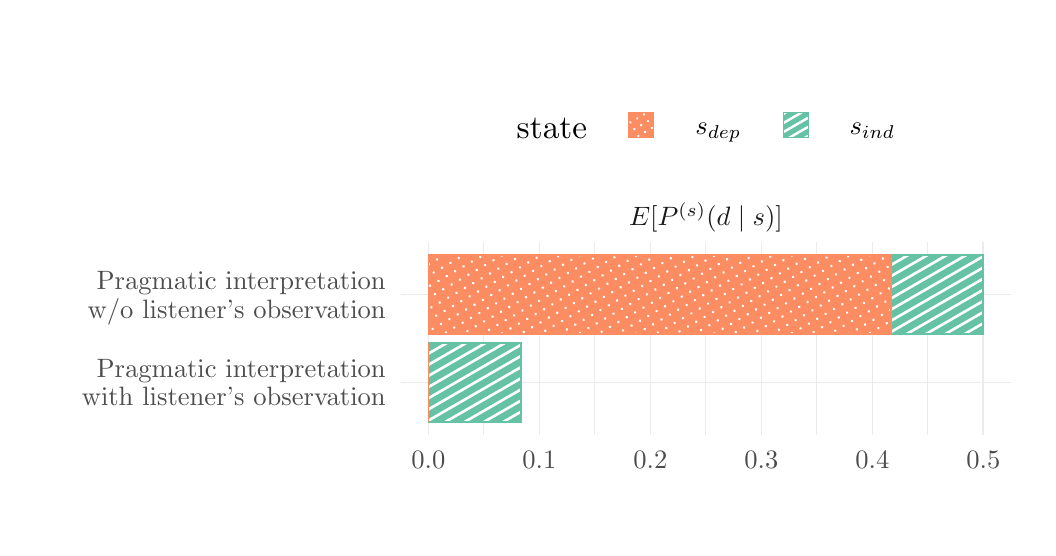
\begin{tikzpicture}[x=1pt,y=1pt]
\definecolor{fillColor}{RGB}{255,255,255}
\path[use as bounding box,fill=fillColor,fill opacity=0.00] (0,0) rectangle (361.35,180.67);
\begin{scope}
\path[clip] (134.78, 33.48) rectangle (355.35,103.28);
\definecolor{drawColor}{gray}{0.92}

\path[draw=drawColor,line width= 0.3pt,line join=round] (164.86, 33.48) --
	(164.86,103.28);

\path[draw=drawColor,line width= 0.3pt,line join=round] (204.96, 33.48) --
	(204.96,103.28);

\path[draw=drawColor,line width= 0.3pt,line join=round] (245.07, 33.48) --
	(245.07,103.28);

\path[draw=drawColor,line width= 0.3pt,line join=round] (285.17, 33.48) --
	(285.17,103.28);

\path[draw=drawColor,line width= 0.3pt,line join=round] (325.27, 33.48) --
	(325.27,103.28);

\path[draw=drawColor,line width= 0.6pt,line join=round] (134.78, 52.51) --
	(355.35, 52.51);

\path[draw=drawColor,line width= 0.6pt,line join=round] (134.78, 84.24) --
	(355.35, 84.24);

\path[draw=drawColor,line width= 0.6pt,line join=round] (144.81, 33.48) --
	(144.81,103.28);

\path[draw=drawColor,line width= 0.6pt,line join=round] (184.91, 33.48) --
	(184.91,103.28);

\path[draw=drawColor,line width= 0.6pt,line join=round] (225.02, 33.48) --
	(225.02,103.28);

\path[draw=drawColor,line width= 0.6pt,line join=round] (265.12, 33.48) --
	(265.12,103.28);

\path[draw=drawColor,line width= 0.6pt,line join=round] (305.22, 33.48) --
	(305.22,103.28);

\path[draw=drawColor,line width= 0.6pt,line join=round] (345.32, 33.48) --
	(345.32,103.28);
\definecolor{fillColor}{RGB}{102,194,165}

\path[fill=fillColor] (311.91, 69.97) rectangle (345.32, 98.52);
\definecolor{fillColor}{RGB}{252,141,98}

\path[fill=fillColor] (144.81, 69.97) rectangle (311.91, 98.52);
\definecolor{fillColor}{RGB}{102,194,165}

\path[fill=fillColor] (144.81, 38.23) rectangle (178.23, 66.79);
\definecolor{fillColor}{RGB}{252,141,98}

\path[fill=fillColor] (144.81, 38.23) rectangle (144.81, 66.79);
\definecolor{drawColor}{RGB}{255,255,255}
\definecolor{fillColor}{RGB}{255,255,255}

\path[draw=drawColor,line width= 0.6pt,line join=round,line cap=rect,fill=fillColor] (345.20, 69.97) --
	(345.32, 70.04) --
	(345.32, 69.97) --
	(345.20, 69.97) --
	cycle;

\path[draw=drawColor,line width= 0.6pt,line join=round,line cap=rect,fill=fillColor] (338.22, 69.97) --
	(345.32, 74.07) --
	(345.32, 73.67) --
	(338.91, 69.97) --
	(338.22, 69.97) --
	cycle;

\path[draw=drawColor,line width= 0.6pt,line join=round,line cap=rect,fill=fillColor] (331.24, 69.97) --
	(345.32, 78.10) --
	(345.32, 77.70) --
	(331.93, 69.97) --
	(331.24, 69.97) --
	cycle;

\path[draw=drawColor,line width= 0.6pt,line join=round,line cap=rect,fill=fillColor] (324.25, 69.97) --
	(345.32, 82.13) --
	(345.32, 81.73) --
	(324.95, 69.97) --
	(324.25, 69.97) --
	cycle;

\path[draw=drawColor,line width= 0.6pt,line join=round,line cap=rect,fill=fillColor] (317.27, 69.97) --
	(345.32, 86.16) --
	(345.32, 85.76) --
	(317.97, 69.97) --
	(317.27, 69.97) --
	cycle;

\path[draw=drawColor,line width= 0.6pt,line join=round,line cap=rect,fill=fillColor] (311.91, 70.90) --
	(345.32, 90.19) --
	(345.32, 89.79) --
	(311.91, 70.49) --
	(311.91, 70.90) --
	cycle;

\path[draw=drawColor,line width= 0.6pt,line join=round,line cap=rect,fill=fillColor] (311.91, 74.93) --
	(345.32, 94.22) --
	(345.32, 93.82) --
	(311.91, 74.52) --
	(311.91, 74.93) --
	cycle;

\path[draw=drawColor,line width= 0.6pt,line join=round,line cap=rect,fill=fillColor] (311.91, 78.96) --
	(345.32, 98.25) --
	(345.32, 97.85) --
	(311.91, 78.55) --
	(311.91, 78.96) --
	cycle;

\path[draw=drawColor,line width= 0.6pt,line join=round,line cap=rect,fill=fillColor] (311.91, 82.99) --
	(338.81, 98.52) --
	(339.51, 98.52) --
	(311.91, 82.58) --
	(311.91, 82.99) --
	cycle;

\path[draw=drawColor,line width= 0.6pt,line join=round,line cap=rect,fill=fillColor] (311.91, 87.02) --
	(331.83, 98.52) --
	(332.53, 98.52) --
	(311.91, 86.61) --
	(311.91, 87.02) --
	cycle;

\path[draw=drawColor,line width= 0.6pt,line join=round,line cap=rect,fill=fillColor] (311.91, 91.05) --
	(324.85, 98.52) --
	(325.55, 98.52) --
	(311.91, 90.65) --
	(311.91, 91.05) --
	cycle;

\path[draw=drawColor,line width= 0.6pt,line join=round,line cap=rect,fill=fillColor] (311.91, 95.08) --
	(317.87, 98.52) --
	(318.57, 98.52) --
	(311.91, 94.68) --
	(311.91, 95.08) --
	cycle;

\path[draw=drawColor,line width= 0.6pt,dash pattern=on 2pt off 2pt ,line join=round,line cap=round,fill=fillColor] (145.41, 87.42) circle (  0.17);

\path[draw=drawColor,line width= 0.6pt,dash pattern=on 2pt off 2pt ,line join=round,line cap=round,fill=fillColor] (145.88, 79.63) circle (  0.17);

\path[draw=drawColor,line width= 0.6pt,dash pattern=on 2pt off 2pt ,line join=round,line cap=round,fill=fillColor] (146.34, 71.84) circle (  0.17);

\path[draw=drawColor,line width= 0.6pt,dash pattern=on 2pt off 2pt ,line join=round,line cap=round,fill=fillColor] (146.69, 92.19) circle (  0.17);

\path[draw=drawColor,line width= 0.6pt,dash pattern=on 2pt off 2pt ,line join=round,line cap=round,fill=fillColor] (147.15, 84.39) circle (  0.17);

\path[draw=drawColor,line width= 0.6pt,dash pattern=on 2pt off 2pt ,line join=round,line cap=round,fill=fillColor] (147.62, 76.60) circle (  0.17);

\path[draw=drawColor,line width= 0.6pt,dash pattern=on 2pt off 2pt ,line join=round,line cap=round,fill=fillColor] (147.96, 96.95) circle (  0.17);

\path[draw=drawColor,line width= 0.6pt,dash pattern=on 2pt off 2pt ,line join=round,line cap=round,fill=fillColor] (148.43, 89.16) circle (  0.17);

\path[draw=drawColor,line width= 0.6pt,dash pattern=on 2pt off 2pt ,line join=round,line cap=round,fill=fillColor] (148.90, 81.37) circle (  0.17);

\path[draw=drawColor,line width= 0.6pt,dash pattern=on 2pt off 2pt ,line join=round,line cap=round,fill=fillColor] (149.37, 73.58) circle (  0.17);

\path[draw=drawColor,line width= 0.6pt,dash pattern=on 2pt off 2pt ,line join=round,line cap=round,fill=fillColor] (149.71, 93.93) circle (  0.17);

\path[draw=drawColor,line width= 0.6pt,dash pattern=on 2pt off 2pt ,line join=round,line cap=round,fill=fillColor] (150.18, 86.14) circle (  0.17);

\path[draw=drawColor,line width= 0.6pt,dash pattern=on 2pt off 2pt ,line join=round,line cap=round,fill=fillColor] (150.64, 78.35) circle (  0.17);

\path[draw=drawColor,line width= 0.6pt,dash pattern=on 2pt off 2pt ,line join=round,line cap=round,fill=fillColor] (151.11, 70.56) circle (  0.17);

\path[draw=drawColor,line width= 0.6pt,dash pattern=on 2pt off 2pt ,line join=round,line cap=round,fill=fillColor] (151.45, 90.91) circle (  0.17);

\path[draw=drawColor,line width= 0.6pt,dash pattern=on 2pt off 2pt ,line join=round,line cap=round,fill=fillColor] (151.92, 83.12) circle (  0.17);

\path[draw=drawColor,line width= 0.6pt,dash pattern=on 2pt off 2pt ,line join=round,line cap=round,fill=fillColor] (152.39, 75.33) circle (  0.17);

\path[draw=drawColor,line width= 0.6pt,dash pattern=on 2pt off 2pt ,line join=round,line cap=round,fill=fillColor] (152.73, 95.68) circle (  0.17);

\path[draw=drawColor,line width= 0.6pt,dash pattern=on 2pt off 2pt ,line join=round,line cap=round,fill=fillColor] (153.20, 87.88) circle (  0.17);

\path[draw=drawColor,line width= 0.6pt,dash pattern=on 2pt off 2pt ,line join=round,line cap=round,fill=fillColor] (153.67, 80.09) circle (  0.17);

\path[draw=drawColor,line width= 0.6pt,dash pattern=on 2pt off 2pt ,line join=round,line cap=round,fill=fillColor] (154.13, 72.30) circle (  0.17);

\path[draw=drawColor,line width= 0.6pt,dash pattern=on 2pt off 2pt ,line join=round,line cap=round,fill=fillColor] (154.48, 92.65) circle (  0.17);

\path[draw=drawColor,line width= 0.6pt,dash pattern=on 2pt off 2pt ,line join=round,line cap=round,fill=fillColor] (154.94, 84.86) circle (  0.17);

\path[draw=drawColor,line width= 0.6pt,dash pattern=on 2pt off 2pt ,line join=round,line cap=round,fill=fillColor] (155.41, 77.07) circle (  0.17);

\path[draw=drawColor,line width= 0.6pt,dash pattern=on 2pt off 2pt ,line join=round,line cap=round,fill=fillColor] (155.75, 97.42) circle (  0.17);

\path[draw=drawColor,line width= 0.6pt,dash pattern=on 2pt off 2pt ,line join=round,line cap=round,fill=fillColor] (156.22, 89.63) circle (  0.17);

\path[draw=drawColor,line width= 0.6pt,dash pattern=on 2pt off 2pt ,line join=round,line cap=round,fill=fillColor] (156.69, 81.84) circle (  0.17);

\path[draw=drawColor,line width= 0.6pt,dash pattern=on 2pt off 2pt ,line join=round,line cap=round,fill=fillColor] (157.16, 74.05) circle (  0.17);

\path[draw=drawColor,line width= 0.6pt,dash pattern=on 2pt off 2pt ,line join=round,line cap=round,fill=fillColor] (157.50, 94.40) circle (  0.17);

\path[draw=drawColor,line width= 0.6pt,dash pattern=on 2pt off 2pt ,line join=round,line cap=round,fill=fillColor] (157.97, 86.61) circle (  0.17);

\path[draw=drawColor,line width= 0.6pt,dash pattern=on 2pt off 2pt ,line join=round,line cap=round,fill=fillColor] (158.43, 78.82) circle (  0.17);

\path[draw=drawColor,line width= 0.6pt,dash pattern=on 2pt off 2pt ,line join=round,line cap=round,fill=fillColor] (158.90, 71.03) circle (  0.17);

\path[draw=drawColor,line width= 0.6pt,dash pattern=on 2pt off 2pt ,line join=round,line cap=round,fill=fillColor] (159.24, 91.38) circle (  0.17);

\path[draw=drawColor,line width= 0.6pt,dash pattern=on 2pt off 2pt ,line join=round,line cap=round,fill=fillColor] (159.71, 83.58) circle (  0.17);

\path[draw=drawColor,line width= 0.6pt,dash pattern=on 2pt off 2pt ,line join=round,line cap=round,fill=fillColor] (160.18, 75.79) circle (  0.17);

\path[draw=drawColor,line width= 0.6pt,dash pattern=on 2pt off 2pt ,line join=round,line cap=round,fill=fillColor] (160.52, 96.14) circle (  0.17);

\path[draw=drawColor,line width= 0.6pt,dash pattern=on 2pt off 2pt ,line join=round,line cap=round,fill=fillColor] (160.99, 88.35) circle (  0.17);

\path[draw=drawColor,line width= 0.6pt,dash pattern=on 2pt off 2pt ,line join=round,line cap=round,fill=fillColor] (161.46, 80.56) circle (  0.17);

\path[draw=drawColor,line width= 0.6pt,dash pattern=on 2pt off 2pt ,line join=round,line cap=round,fill=fillColor] (161.92, 72.77) circle (  0.17);

\path[draw=drawColor,line width= 0.6pt,dash pattern=on 2pt off 2pt ,line join=round,line cap=round,fill=fillColor] (162.27, 93.12) circle (  0.17);

\path[draw=drawColor,line width= 0.6pt,dash pattern=on 2pt off 2pt ,line join=round,line cap=round,fill=fillColor] (162.73, 85.33) circle (  0.17);

\path[draw=drawColor,line width= 0.6pt,dash pattern=on 2pt off 2pt ,line join=round,line cap=round,fill=fillColor] (163.20, 77.54) circle (  0.17);

\path[draw=drawColor,line width= 0.6pt,dash pattern=on 2pt off 2pt ,line join=round,line cap=round,fill=fillColor] (163.54, 97.89) circle (  0.17);

\path[draw=drawColor,line width= 0.6pt,dash pattern=on 2pt off 2pt ,line join=round,line cap=round,fill=fillColor] (164.01, 90.10) circle (  0.17);

\path[draw=drawColor,line width= 0.6pt,dash pattern=on 2pt off 2pt ,line join=round,line cap=round,fill=fillColor] (164.48, 82.31) circle (  0.17);

\path[draw=drawColor,line width= 0.6pt,dash pattern=on 2pt off 2pt ,line join=round,line cap=round,fill=fillColor] (164.95, 74.52) circle (  0.17);

\path[draw=drawColor,line width= 0.6pt,dash pattern=on 2pt off 2pt ,line join=round,line cap=round,fill=fillColor] (165.29, 94.87) circle (  0.17);

\path[draw=drawColor,line width= 0.6pt,dash pattern=on 2pt off 2pt ,line join=round,line cap=round,fill=fillColor] (165.76, 87.07) circle (  0.17);

\path[draw=drawColor,line width= 0.6pt,dash pattern=on 2pt off 2pt ,line join=round,line cap=round,fill=fillColor] (166.23, 79.28) circle (  0.17);

\path[draw=drawColor,line width= 0.6pt,dash pattern=on 2pt off 2pt ,line join=round,line cap=round,fill=fillColor] (166.69, 71.49) circle (  0.17);

\path[draw=drawColor,line width= 0.6pt,dash pattern=on 2pt off 2pt ,line join=round,line cap=round,fill=fillColor] (167.04, 91.84) circle (  0.17);

\path[draw=drawColor,line width= 0.6pt,dash pattern=on 2pt off 2pt ,line join=round,line cap=round,fill=fillColor] (167.50, 84.05) circle (  0.17);

\path[draw=drawColor,line width= 0.6pt,dash pattern=on 2pt off 2pt ,line join=round,line cap=round,fill=fillColor] (167.97, 76.26) circle (  0.17);

\path[draw=drawColor,line width= 0.6pt,dash pattern=on 2pt off 2pt ,line join=round,line cap=round,fill=fillColor] (168.31, 96.61) circle (  0.17);

\path[draw=drawColor,line width= 0.6pt,dash pattern=on 2pt off 2pt ,line join=round,line cap=round,fill=fillColor] (168.78, 88.82) circle (  0.17);

\path[draw=drawColor,line width= 0.6pt,dash pattern=on 2pt off 2pt ,line join=round,line cap=round,fill=fillColor] (169.25, 81.03) circle (  0.17);

\path[draw=drawColor,line width= 0.6pt,dash pattern=on 2pt off 2pt ,line join=round,line cap=round,fill=fillColor] (169.72, 73.24) circle (  0.17);

\path[draw=drawColor,line width= 0.6pt,dash pattern=on 2pt off 2pt ,line join=round,line cap=round,fill=fillColor] (170.06, 93.59) circle (  0.17);

\path[draw=drawColor,line width= 0.6pt,dash pattern=on 2pt off 2pt ,line join=round,line cap=round,fill=fillColor] (170.53, 85.80) circle (  0.17);

\path[draw=drawColor,line width= 0.6pt,dash pattern=on 2pt off 2pt ,line join=round,line cap=round,fill=fillColor] (170.99, 78.01) circle (  0.17);

\path[draw=drawColor,line width= 0.6pt,dash pattern=on 2pt off 2pt ,line join=round,line cap=round,fill=fillColor] (171.46, 70.22) circle (  0.17);

\path[draw=drawColor,line width= 0.6pt,dash pattern=on 2pt off 2pt ,line join=round,line cap=round,fill=fillColor] (171.80, 90.57) circle (  0.17);

\path[draw=drawColor,line width= 0.6pt,dash pattern=on 2pt off 2pt ,line join=round,line cap=round,fill=fillColor] (172.27, 82.77) circle (  0.17);

\path[draw=drawColor,line width= 0.6pt,dash pattern=on 2pt off 2pt ,line join=round,line cap=round,fill=fillColor] (172.74, 74.98) circle (  0.17);

\path[draw=drawColor,line width= 0.6pt,dash pattern=on 2pt off 2pt ,line join=round,line cap=round,fill=fillColor] (173.08, 95.33) circle (  0.17);

\path[draw=drawColor,line width= 0.6pt,dash pattern=on 2pt off 2pt ,line join=round,line cap=round,fill=fillColor] (173.55, 87.54) circle (  0.17);

\path[draw=drawColor,line width= 0.6pt,dash pattern=on 2pt off 2pt ,line join=round,line cap=round,fill=fillColor] (174.02, 79.75) circle (  0.17);

\path[draw=drawColor,line width= 0.6pt,dash pattern=on 2pt off 2pt ,line join=round,line cap=round,fill=fillColor] (174.48, 71.96) circle (  0.17);

\path[draw=drawColor,line width= 0.6pt,dash pattern=on 2pt off 2pt ,line join=round,line cap=round,fill=fillColor] (174.83, 92.31) circle (  0.17);

\path[draw=drawColor,line width= 0.6pt,dash pattern=on 2pt off 2pt ,line join=round,line cap=round,fill=fillColor] (175.29, 84.52) circle (  0.17);

\path[draw=drawColor,line width= 0.6pt,dash pattern=on 2pt off 2pt ,line join=round,line cap=round,fill=fillColor] (175.76, 76.73) circle (  0.17);

\path[draw=drawColor,line width= 0.6pt,dash pattern=on 2pt off 2pt ,line join=round,line cap=round,fill=fillColor] (176.10, 97.08) circle (  0.17);

\path[draw=drawColor,line width= 0.6pt,dash pattern=on 2pt off 2pt ,line join=round,line cap=round,fill=fillColor] (176.57, 89.29) circle (  0.17);

\path[draw=drawColor,line width= 0.6pt,dash pattern=on 2pt off 2pt ,line join=round,line cap=round,fill=fillColor] (177.04, 81.50) circle (  0.17);

\path[draw=drawColor,line width= 0.6pt,dash pattern=on 2pt off 2pt ,line join=round,line cap=round,fill=fillColor] (177.51, 73.71) circle (  0.17);

\path[draw=drawColor,line width= 0.6pt,dash pattern=on 2pt off 2pt ,line join=round,line cap=round,fill=fillColor] (177.85, 94.06) circle (  0.17);

\path[draw=drawColor,line width= 0.6pt,dash pattern=on 2pt off 2pt ,line join=round,line cap=round,fill=fillColor] (178.32, 86.26) circle (  0.17);

\path[draw=drawColor,line width= 0.6pt,dash pattern=on 2pt off 2pt ,line join=round,line cap=round,fill=fillColor] (178.78, 78.47) circle (  0.17);

\path[draw=drawColor,line width= 0.6pt,dash pattern=on 2pt off 2pt ,line join=round,line cap=round,fill=fillColor] (179.25, 70.68) circle (  0.17);

\path[draw=drawColor,line width= 0.6pt,dash pattern=on 2pt off 2pt ,line join=round,line cap=round,fill=fillColor] (179.59, 91.03) circle (  0.17);

\path[draw=drawColor,line width= 0.6pt,dash pattern=on 2pt off 2pt ,line join=round,line cap=round,fill=fillColor] (180.06, 83.24) circle (  0.17);

\path[draw=drawColor,line width= 0.6pt,dash pattern=on 2pt off 2pt ,line join=round,line cap=round,fill=fillColor] (180.53, 75.45) circle (  0.17);

\path[draw=drawColor,line width= 0.6pt,dash pattern=on 2pt off 2pt ,line join=round,line cap=round,fill=fillColor] (180.87, 95.80) circle (  0.17);

\path[draw=drawColor,line width= 0.6pt,dash pattern=on 2pt off 2pt ,line join=round,line cap=round,fill=fillColor] (181.34, 88.01) circle (  0.17);

\path[draw=drawColor,line width= 0.6pt,dash pattern=on 2pt off 2pt ,line join=round,line cap=round,fill=fillColor] (181.81, 80.22) circle (  0.17);

\path[draw=drawColor,line width= 0.6pt,dash pattern=on 2pt off 2pt ,line join=round,line cap=round,fill=fillColor] (182.27, 72.43) circle (  0.17);

\path[draw=drawColor,line width= 0.6pt,dash pattern=on 2pt off 2pt ,line join=round,line cap=round,fill=fillColor] (182.62, 92.78) circle (  0.17);

\path[draw=drawColor,line width= 0.6pt,dash pattern=on 2pt off 2pt ,line join=round,line cap=round,fill=fillColor] (183.08, 84.99) circle (  0.17);

\path[draw=drawColor,line width= 0.6pt,dash pattern=on 2pt off 2pt ,line join=round,line cap=round,fill=fillColor] (183.55, 77.20) circle (  0.17);

\path[draw=drawColor,line width= 0.6pt,dash pattern=on 2pt off 2pt ,line join=round,line cap=round,fill=fillColor] (183.89, 97.55) circle (  0.17);

\path[draw=drawColor,line width= 0.6pt,dash pattern=on 2pt off 2pt ,line join=round,line cap=round,fill=fillColor] (184.36, 89.76) circle (  0.17);

\path[draw=drawColor,line width= 0.6pt,dash pattern=on 2pt off 2pt ,line join=round,line cap=round,fill=fillColor] (184.83, 81.96) circle (  0.17);

\path[draw=drawColor,line width= 0.6pt,dash pattern=on 2pt off 2pt ,line join=round,line cap=round,fill=fillColor] (185.30, 74.17) circle (  0.17);

\path[draw=drawColor,line width= 0.6pt,dash pattern=on 2pt off 2pt ,line join=round,line cap=round,fill=fillColor] (185.64, 94.52) circle (  0.17);

\path[draw=drawColor,line width= 0.6pt,dash pattern=on 2pt off 2pt ,line join=round,line cap=round,fill=fillColor] (186.11, 86.73) circle (  0.17);

\path[draw=drawColor,line width= 0.6pt,dash pattern=on 2pt off 2pt ,line join=round,line cap=round,fill=fillColor] (186.57, 78.94) circle (  0.17);

\path[draw=drawColor,line width= 0.6pt,dash pattern=on 2pt off 2pt ,line join=round,line cap=round,fill=fillColor] (187.04, 71.15) circle (  0.17);

\path[draw=drawColor,line width= 0.6pt,dash pattern=on 2pt off 2pt ,line join=round,line cap=round,fill=fillColor] (187.38, 91.50) circle (  0.17);

\path[draw=drawColor,line width= 0.6pt,dash pattern=on 2pt off 2pt ,line join=round,line cap=round,fill=fillColor] (187.85, 83.71) circle (  0.17);

\path[draw=drawColor,line width= 0.6pt,dash pattern=on 2pt off 2pt ,line join=round,line cap=round,fill=fillColor] (188.32, 75.92) circle (  0.17);

\path[draw=drawColor,line width= 0.6pt,dash pattern=on 2pt off 2pt ,line join=round,line cap=round,fill=fillColor] (188.66, 96.27) circle (  0.17);

\path[draw=drawColor,line width= 0.6pt,dash pattern=on 2pt off 2pt ,line join=round,line cap=round,fill=fillColor] (189.13, 88.48) circle (  0.17);

\path[draw=drawColor,line width= 0.6pt,dash pattern=on 2pt off 2pt ,line join=round,line cap=round,fill=fillColor] (189.60, 80.69) circle (  0.17);

\path[draw=drawColor,line width= 0.6pt,dash pattern=on 2pt off 2pt ,line join=round,line cap=round,fill=fillColor] (190.06, 72.90) circle (  0.17);

\path[draw=drawColor,line width= 0.6pt,dash pattern=on 2pt off 2pt ,line join=round,line cap=round,fill=fillColor] (190.41, 93.25) circle (  0.17);

\path[draw=drawColor,line width= 0.6pt,dash pattern=on 2pt off 2pt ,line join=round,line cap=round,fill=fillColor] (190.87, 85.46) circle (  0.17);

\path[draw=drawColor,line width= 0.6pt,dash pattern=on 2pt off 2pt ,line join=round,line cap=round,fill=fillColor] (191.34, 77.66) circle (  0.17);

\path[draw=drawColor,line width= 0.6pt,dash pattern=on 2pt off 2pt ,line join=round,line cap=round,fill=fillColor] (191.68, 98.01) circle (  0.17);

\path[draw=drawColor,line width= 0.6pt,dash pattern=on 2pt off 2pt ,line join=round,line cap=round,fill=fillColor] (192.15, 90.22) circle (  0.17);

\path[draw=drawColor,line width= 0.6pt,dash pattern=on 2pt off 2pt ,line join=round,line cap=round,fill=fillColor] (192.62, 82.43) circle (  0.17);

\path[draw=drawColor,line width= 0.6pt,dash pattern=on 2pt off 2pt ,line join=round,line cap=round,fill=fillColor] (193.09, 74.64) circle (  0.17);

\path[draw=drawColor,line width= 0.6pt,dash pattern=on 2pt off 2pt ,line join=round,line cap=round,fill=fillColor] (193.43, 94.99) circle (  0.17);

\path[draw=drawColor,line width= 0.6pt,dash pattern=on 2pt off 2pt ,line join=round,line cap=round,fill=fillColor] (193.90, 87.20) circle (  0.17);

\path[draw=drawColor,line width= 0.6pt,dash pattern=on 2pt off 2pt ,line join=round,line cap=round,fill=fillColor] (194.37, 79.41) circle (  0.17);

\path[draw=drawColor,line width= 0.6pt,dash pattern=on 2pt off 2pt ,line join=round,line cap=round,fill=fillColor] (194.83, 71.62) circle (  0.17);

\path[draw=drawColor,line width= 0.6pt,dash pattern=on 2pt off 2pt ,line join=round,line cap=round,fill=fillColor] (195.18, 91.97) circle (  0.17);

\path[draw=drawColor,line width= 0.6pt,dash pattern=on 2pt off 2pt ,line join=round,line cap=round,fill=fillColor] (195.64, 84.18) circle (  0.17);

\path[draw=drawColor,line width= 0.6pt,dash pattern=on 2pt off 2pt ,line join=round,line cap=round,fill=fillColor] (196.11, 76.39) circle (  0.17);

\path[draw=drawColor,line width= 0.6pt,dash pattern=on 2pt off 2pt ,line join=round,line cap=round,fill=fillColor] (196.45, 96.74) circle (  0.17);

\path[draw=drawColor,line width= 0.6pt,dash pattern=on 2pt off 2pt ,line join=round,line cap=round,fill=fillColor] (196.92, 88.95) circle (  0.17);

\path[draw=drawColor,line width= 0.6pt,dash pattern=on 2pt off 2pt ,line join=round,line cap=round,fill=fillColor] (197.39, 81.15) circle (  0.17);

\path[draw=drawColor,line width= 0.6pt,dash pattern=on 2pt off 2pt ,line join=round,line cap=round,fill=fillColor] (197.86, 73.36) circle (  0.17);

\path[draw=drawColor,line width= 0.6pt,dash pattern=on 2pt off 2pt ,line join=round,line cap=round,fill=fillColor] (198.20, 93.71) circle (  0.17);

\path[draw=drawColor,line width= 0.6pt,dash pattern=on 2pt off 2pt ,line join=round,line cap=round,fill=fillColor] (198.67, 85.92) circle (  0.17);

\path[draw=drawColor,line width= 0.6pt,dash pattern=on 2pt off 2pt ,line join=round,line cap=round,fill=fillColor] (199.13, 78.13) circle (  0.17);

\path[draw=drawColor,line width= 0.6pt,dash pattern=on 2pt off 2pt ,line join=round,line cap=round,fill=fillColor] (199.60, 70.34) circle (  0.17);

\path[draw=drawColor,line width= 0.6pt,dash pattern=on 2pt off 2pt ,line join=round,line cap=round,fill=fillColor] (199.94, 90.69) circle (  0.17);

\path[draw=drawColor,line width= 0.6pt,dash pattern=on 2pt off 2pt ,line join=round,line cap=round,fill=fillColor] (200.41, 82.90) circle (  0.17);

\path[draw=drawColor,line width= 0.6pt,dash pattern=on 2pt off 2pt ,line join=round,line cap=round,fill=fillColor] (200.88, 75.11) circle (  0.17);

\path[draw=drawColor,line width= 0.6pt,dash pattern=on 2pt off 2pt ,line join=round,line cap=round,fill=fillColor] (201.22, 95.46) circle (  0.17);

\path[draw=drawColor,line width= 0.6pt,dash pattern=on 2pt off 2pt ,line join=round,line cap=round,fill=fillColor] (201.69, 87.67) circle (  0.17);

\path[draw=drawColor,line width= 0.6pt,dash pattern=on 2pt off 2pt ,line join=round,line cap=round,fill=fillColor] (202.16, 79.88) circle (  0.17);

\path[draw=drawColor,line width= 0.6pt,dash pattern=on 2pt off 2pt ,line join=round,line cap=round,fill=fillColor] (202.62, 72.09) circle (  0.17);

\path[draw=drawColor,line width= 0.6pt,dash pattern=on 2pt off 2pt ,line join=round,line cap=round,fill=fillColor] (202.97, 92.44) circle (  0.17);

\path[draw=drawColor,line width= 0.6pt,dash pattern=on 2pt off 2pt ,line join=round,line cap=round,fill=fillColor] (203.43, 84.65) circle (  0.17);

\path[draw=drawColor,line width= 0.6pt,dash pattern=on 2pt off 2pt ,line join=round,line cap=round,fill=fillColor] (203.90, 76.85) circle (  0.17);

\path[draw=drawColor,line width= 0.6pt,dash pattern=on 2pt off 2pt ,line join=round,line cap=round,fill=fillColor] (204.24, 97.20) circle (  0.17);

\path[draw=drawColor,line width= 0.6pt,dash pattern=on 2pt off 2pt ,line join=round,line cap=round,fill=fillColor] (204.71, 89.41) circle (  0.17);

\path[draw=drawColor,line width= 0.6pt,dash pattern=on 2pt off 2pt ,line join=round,line cap=round,fill=fillColor] (205.18, 81.62) circle (  0.17);

\path[draw=drawColor,line width= 0.6pt,dash pattern=on 2pt off 2pt ,line join=round,line cap=round,fill=fillColor] (205.65, 73.83) circle (  0.17);

\path[draw=drawColor,line width= 0.6pt,dash pattern=on 2pt off 2pt ,line join=round,line cap=round,fill=fillColor] (205.99, 94.18) circle (  0.17);

\path[draw=drawColor,line width= 0.6pt,dash pattern=on 2pt off 2pt ,line join=round,line cap=round,fill=fillColor] (206.46, 86.39) circle (  0.17);

\path[draw=drawColor,line width= 0.6pt,dash pattern=on 2pt off 2pt ,line join=round,line cap=round,fill=fillColor] (206.92, 78.60) circle (  0.17);

\path[draw=drawColor,line width= 0.6pt,dash pattern=on 2pt off 2pt ,line join=round,line cap=round,fill=fillColor] (207.39, 70.81) circle (  0.17);

\path[draw=drawColor,line width= 0.6pt,dash pattern=on 2pt off 2pt ,line join=round,line cap=round,fill=fillColor] (207.73, 91.16) circle (  0.17);

\path[draw=drawColor,line width= 0.6pt,dash pattern=on 2pt off 2pt ,line join=round,line cap=round,fill=fillColor] (208.20, 83.37) circle (  0.17);

\path[draw=drawColor,line width= 0.6pt,dash pattern=on 2pt off 2pt ,line join=round,line cap=round,fill=fillColor] (208.67, 75.58) circle (  0.17);

\path[draw=drawColor,line width= 0.6pt,dash pattern=on 2pt off 2pt ,line join=round,line cap=round,fill=fillColor] (209.01, 95.93) circle (  0.17);

\path[draw=drawColor,line width= 0.6pt,dash pattern=on 2pt off 2pt ,line join=round,line cap=round,fill=fillColor] (209.48, 88.14) circle (  0.17);

\path[draw=drawColor,line width= 0.6pt,dash pattern=on 2pt off 2pt ,line join=round,line cap=round,fill=fillColor] (209.95, 80.34) circle (  0.17);

\path[draw=drawColor,line width= 0.6pt,dash pattern=on 2pt off 2pt ,line join=round,line cap=round,fill=fillColor] (210.41, 72.55) circle (  0.17);

\path[draw=drawColor,line width= 0.6pt,dash pattern=on 2pt off 2pt ,line join=round,line cap=round,fill=fillColor] (210.76, 92.90) circle (  0.17);

\path[draw=drawColor,line width= 0.6pt,dash pattern=on 2pt off 2pt ,line join=round,line cap=round,fill=fillColor] (211.22, 85.11) circle (  0.17);

\path[draw=drawColor,line width= 0.6pt,dash pattern=on 2pt off 2pt ,line join=round,line cap=round,fill=fillColor] (211.69, 77.32) circle (  0.17);

\path[draw=drawColor,line width= 0.6pt,dash pattern=on 2pt off 2pt ,line join=round,line cap=round,fill=fillColor] (212.03, 97.67) circle (  0.17);

\path[draw=drawColor,line width= 0.6pt,dash pattern=on 2pt off 2pt ,line join=round,line cap=round,fill=fillColor] (212.50, 89.88) circle (  0.17);

\path[draw=drawColor,line width= 0.6pt,dash pattern=on 2pt off 2pt ,line join=round,line cap=round,fill=fillColor] (212.97, 82.09) circle (  0.17);

\path[draw=drawColor,line width= 0.6pt,dash pattern=on 2pt off 2pt ,line join=round,line cap=round,fill=fillColor] (213.44, 74.30) circle (  0.17);

\path[draw=drawColor,line width= 0.6pt,dash pattern=on 2pt off 2pt ,line join=round,line cap=round,fill=fillColor] (213.78, 94.65) circle (  0.17);

\path[draw=drawColor,line width= 0.6pt,dash pattern=on 2pt off 2pt ,line join=round,line cap=round,fill=fillColor] (214.25, 86.86) circle (  0.17);

\path[draw=drawColor,line width= 0.6pt,dash pattern=on 2pt off 2pt ,line join=round,line cap=round,fill=fillColor] (214.71, 79.07) circle (  0.17);

\path[draw=drawColor,line width= 0.6pt,dash pattern=on 2pt off 2pt ,line join=round,line cap=round,fill=fillColor] (215.18, 71.28) circle (  0.17);

\path[draw=drawColor,line width= 0.6pt,dash pattern=on 2pt off 2pt ,line join=round,line cap=round,fill=fillColor] (215.52, 91.63) circle (  0.17);

\path[draw=drawColor,line width= 0.6pt,dash pattern=on 2pt off 2pt ,line join=round,line cap=round,fill=fillColor] (215.99, 83.84) circle (  0.17);

\path[draw=drawColor,line width= 0.6pt,dash pattern=on 2pt off 2pt ,line join=round,line cap=round,fill=fillColor] (216.46, 76.04) circle (  0.17);

\path[draw=drawColor,line width= 0.6pt,dash pattern=on 2pt off 2pt ,line join=round,line cap=round,fill=fillColor] (216.80, 96.39) circle (  0.17);

\path[draw=drawColor,line width= 0.6pt,dash pattern=on 2pt off 2pt ,line join=round,line cap=round,fill=fillColor] (217.27, 88.60) circle (  0.17);

\path[draw=drawColor,line width= 0.6pt,dash pattern=on 2pt off 2pt ,line join=round,line cap=round,fill=fillColor] (217.74, 80.81) circle (  0.17);

\path[draw=drawColor,line width= 0.6pt,dash pattern=on 2pt off 2pt ,line join=round,line cap=round,fill=fillColor] (218.20, 73.02) circle (  0.17);

\path[draw=drawColor,line width= 0.6pt,dash pattern=on 2pt off 2pt ,line join=round,line cap=round,fill=fillColor] (218.55, 93.37) circle (  0.17);

\path[draw=drawColor,line width= 0.6pt,dash pattern=on 2pt off 2pt ,line join=round,line cap=round,fill=fillColor] (219.01, 85.58) circle (  0.17);

\path[draw=drawColor,line width= 0.6pt,dash pattern=on 2pt off 2pt ,line join=round,line cap=round,fill=fillColor] (219.48, 77.79) circle (  0.17);

\path[draw=drawColor,line width= 0.6pt,dash pattern=on 2pt off 2pt ,line join=round,line cap=round,fill=fillColor] (219.82, 98.14) circle (  0.17);

\path[draw=drawColor,line width= 0.6pt,dash pattern=on 2pt off 2pt ,line join=round,line cap=round,fill=fillColor] (220.29, 90.35) circle (  0.17);

\path[draw=drawColor,line width= 0.6pt,dash pattern=on 2pt off 2pt ,line join=round,line cap=round,fill=fillColor] (220.76, 82.56) circle (  0.17);

\path[draw=drawColor,line width= 0.6pt,dash pattern=on 2pt off 2pt ,line join=round,line cap=round,fill=fillColor] (221.23, 74.77) circle (  0.17);

\path[draw=drawColor,line width= 0.6pt,dash pattern=on 2pt off 2pt ,line join=round,line cap=round,fill=fillColor] (221.57, 95.12) circle (  0.17);

\path[draw=drawColor,line width= 0.6pt,dash pattern=on 2pt off 2pt ,line join=round,line cap=round,fill=fillColor] (222.04, 87.33) circle (  0.17);

\path[draw=drawColor,line width= 0.6pt,dash pattern=on 2pt off 2pt ,line join=round,line cap=round,fill=fillColor] (222.51, 79.53) circle (  0.17);

\path[draw=drawColor,line width= 0.6pt,dash pattern=on 2pt off 2pt ,line join=round,line cap=round,fill=fillColor] (222.97, 71.74) circle (  0.17);

\path[draw=drawColor,line width= 0.6pt,dash pattern=on 2pt off 2pt ,line join=round,line cap=round,fill=fillColor] (223.32, 92.09) circle (  0.17);

\path[draw=drawColor,line width= 0.6pt,dash pattern=on 2pt off 2pt ,line join=round,line cap=round,fill=fillColor] (223.78, 84.30) circle (  0.17);

\path[draw=drawColor,line width= 0.6pt,dash pattern=on 2pt off 2pt ,line join=round,line cap=round,fill=fillColor] (224.25, 76.51) circle (  0.17);

\path[draw=drawColor,line width= 0.6pt,dash pattern=on 2pt off 2pt ,line join=round,line cap=round,fill=fillColor] (224.59, 96.86) circle (  0.17);

\path[draw=drawColor,line width= 0.6pt,dash pattern=on 2pt off 2pt ,line join=round,line cap=round,fill=fillColor] (225.06, 89.07) circle (  0.17);

\path[draw=drawColor,line width= 0.6pt,dash pattern=on 2pt off 2pt ,line join=round,line cap=round,fill=fillColor] (225.53, 81.28) circle (  0.17);

\path[draw=drawColor,line width= 0.6pt,dash pattern=on 2pt off 2pt ,line join=round,line cap=round,fill=fillColor] (226.00, 73.49) circle (  0.17);

\path[draw=drawColor,line width= 0.6pt,dash pattern=on 2pt off 2pt ,line join=round,line cap=round,fill=fillColor] (226.34, 93.84) circle (  0.17);

\path[draw=drawColor,line width= 0.6pt,dash pattern=on 2pt off 2pt ,line join=round,line cap=round,fill=fillColor] (226.81, 86.05) circle (  0.17);

\path[draw=drawColor,line width= 0.6pt,dash pattern=on 2pt off 2pt ,line join=round,line cap=round,fill=fillColor] (227.27, 78.26) circle (  0.17);

\path[draw=drawColor,line width= 0.6pt,dash pattern=on 2pt off 2pt ,line join=round,line cap=round,fill=fillColor] (227.74, 70.47) circle (  0.17);

\path[draw=drawColor,line width= 0.6pt,dash pattern=on 2pt off 2pt ,line join=round,line cap=round,fill=fillColor] (228.08, 90.82) circle (  0.17);

\path[draw=drawColor,line width= 0.6pt,dash pattern=on 2pt off 2pt ,line join=round,line cap=round,fill=fillColor] (228.55, 83.03) circle (  0.17);

\path[draw=drawColor,line width= 0.6pt,dash pattern=on 2pt off 2pt ,line join=round,line cap=round,fill=fillColor] (229.02, 75.23) circle (  0.17);

\path[draw=drawColor,line width= 0.6pt,dash pattern=on 2pt off 2pt ,line join=round,line cap=round,fill=fillColor] (229.36, 95.58) circle (  0.17);

\path[draw=drawColor,line width= 0.6pt,dash pattern=on 2pt off 2pt ,line join=round,line cap=round,fill=fillColor] (229.83, 87.79) circle (  0.17);

\path[draw=drawColor,line width= 0.6pt,dash pattern=on 2pt off 2pt ,line join=round,line cap=round,fill=fillColor] (230.30, 80.00) circle (  0.17);

\path[draw=drawColor,line width= 0.6pt,dash pattern=on 2pt off 2pt ,line join=round,line cap=round,fill=fillColor] (230.76, 72.21) circle (  0.17);

\path[draw=drawColor,line width= 0.6pt,dash pattern=on 2pt off 2pt ,line join=round,line cap=round,fill=fillColor] (231.11, 92.56) circle (  0.17);

\path[draw=drawColor,line width= 0.6pt,dash pattern=on 2pt off 2pt ,line join=round,line cap=round,fill=fillColor] (231.57, 84.77) circle (  0.17);

\path[draw=drawColor,line width= 0.6pt,dash pattern=on 2pt off 2pt ,line join=round,line cap=round,fill=fillColor] (232.04, 76.98) circle (  0.17);

\path[draw=drawColor,line width= 0.6pt,dash pattern=on 2pt off 2pt ,line join=round,line cap=round,fill=fillColor] (232.38, 97.33) circle (  0.17);

\path[draw=drawColor,line width= 0.6pt,dash pattern=on 2pt off 2pt ,line join=round,line cap=round,fill=fillColor] (232.85, 89.54) circle (  0.17);

\path[draw=drawColor,line width= 0.6pt,dash pattern=on 2pt off 2pt ,line join=round,line cap=round,fill=fillColor] (233.32, 81.75) circle (  0.17);

\path[draw=drawColor,line width= 0.6pt,dash pattern=on 2pt off 2pt ,line join=round,line cap=round,fill=fillColor] (233.79, 73.96) circle (  0.17);

\path[draw=drawColor,line width= 0.6pt,dash pattern=on 2pt off 2pt ,line join=round,line cap=round,fill=fillColor] (234.13, 94.31) circle (  0.17);

\path[draw=drawColor,line width= 0.6pt,dash pattern=on 2pt off 2pt ,line join=round,line cap=round,fill=fillColor] (234.60, 86.52) circle (  0.17);

\path[draw=drawColor,line width= 0.6pt,dash pattern=on 2pt off 2pt ,line join=round,line cap=round,fill=fillColor] (235.06, 78.72) circle (  0.17);

\path[draw=drawColor,line width= 0.6pt,dash pattern=on 2pt off 2pt ,line join=round,line cap=round,fill=fillColor] (235.53, 70.93) circle (  0.17);

\path[draw=drawColor,line width= 0.6pt,dash pattern=on 2pt off 2pt ,line join=round,line cap=round,fill=fillColor] (235.87, 91.28) circle (  0.17);

\path[draw=drawColor,line width= 0.6pt,dash pattern=on 2pt off 2pt ,line join=round,line cap=round,fill=fillColor] (236.34, 83.49) circle (  0.17);

\path[draw=drawColor,line width= 0.6pt,dash pattern=on 2pt off 2pt ,line join=round,line cap=round,fill=fillColor] (236.81, 75.70) circle (  0.17);

\path[draw=drawColor,line width= 0.6pt,dash pattern=on 2pt off 2pt ,line join=round,line cap=round,fill=fillColor] (237.15, 96.05) circle (  0.17);

\path[draw=drawColor,line width= 0.6pt,dash pattern=on 2pt off 2pt ,line join=round,line cap=round,fill=fillColor] (237.62, 88.26) circle (  0.17);

\path[draw=drawColor,line width= 0.6pt,dash pattern=on 2pt off 2pt ,line join=round,line cap=round,fill=fillColor] (238.09, 80.47) circle (  0.17);

\path[draw=drawColor,line width= 0.6pt,dash pattern=on 2pt off 2pt ,line join=round,line cap=round,fill=fillColor] (238.55, 72.68) circle (  0.17);

\path[draw=drawColor,line width= 0.6pt,dash pattern=on 2pt off 2pt ,line join=round,line cap=round,fill=fillColor] (238.90, 93.03) circle (  0.17);

\path[draw=drawColor,line width= 0.6pt,dash pattern=on 2pt off 2pt ,line join=round,line cap=round,fill=fillColor] (239.36, 85.24) circle (  0.17);

\path[draw=drawColor,line width= 0.6pt,dash pattern=on 2pt off 2pt ,line join=round,line cap=round,fill=fillColor] (239.83, 77.45) circle (  0.17);

\path[draw=drawColor,line width= 0.6pt,dash pattern=on 2pt off 2pt ,line join=round,line cap=round,fill=fillColor] (240.17, 97.80) circle (  0.17);

\path[draw=drawColor,line width= 0.6pt,dash pattern=on 2pt off 2pt ,line join=round,line cap=round,fill=fillColor] (240.64, 90.01) circle (  0.17);

\path[draw=drawColor,line width= 0.6pt,dash pattern=on 2pt off 2pt ,line join=round,line cap=round,fill=fillColor] (241.11, 82.22) circle (  0.17);

\path[draw=drawColor,line width= 0.6pt,dash pattern=on 2pt off 2pt ,line join=round,line cap=round,fill=fillColor] (241.58, 74.42) circle (  0.17);

\path[draw=drawColor,line width= 0.6pt,dash pattern=on 2pt off 2pt ,line join=round,line cap=round,fill=fillColor] (241.92, 94.77) circle (  0.17);

\path[draw=drawColor,line width= 0.6pt,dash pattern=on 2pt off 2pt ,line join=round,line cap=round,fill=fillColor] (242.39, 86.98) circle (  0.17);

\path[draw=drawColor,line width= 0.6pt,dash pattern=on 2pt off 2pt ,line join=round,line cap=round,fill=fillColor] (242.85, 79.19) circle (  0.17);

\path[draw=drawColor,line width= 0.6pt,dash pattern=on 2pt off 2pt ,line join=round,line cap=round,fill=fillColor] (243.32, 71.40) circle (  0.17);

\path[draw=drawColor,line width= 0.6pt,dash pattern=on 2pt off 2pt ,line join=round,line cap=round,fill=fillColor] (243.66, 91.75) circle (  0.17);

\path[draw=drawColor,line width= 0.6pt,dash pattern=on 2pt off 2pt ,line join=round,line cap=round,fill=fillColor] (244.13, 83.96) circle (  0.17);

\path[draw=drawColor,line width= 0.6pt,dash pattern=on 2pt off 2pt ,line join=round,line cap=round,fill=fillColor] (244.60, 76.17) circle (  0.17);

\path[draw=drawColor,line width= 0.6pt,dash pattern=on 2pt off 2pt ,line join=round,line cap=round,fill=fillColor] (244.94, 96.52) circle (  0.17);

\path[draw=drawColor,line width= 0.6pt,dash pattern=on 2pt off 2pt ,line join=round,line cap=round,fill=fillColor] (245.41, 88.73) circle (  0.17);

\path[draw=drawColor,line width= 0.6pt,dash pattern=on 2pt off 2pt ,line join=round,line cap=round,fill=fillColor] (245.88, 80.94) circle (  0.17);

\path[draw=drawColor,line width= 0.6pt,dash pattern=on 2pt off 2pt ,line join=round,line cap=round,fill=fillColor] (246.34, 73.15) circle (  0.17);

\path[draw=drawColor,line width= 0.6pt,dash pattern=on 2pt off 2pt ,line join=round,line cap=round,fill=fillColor] (246.69, 93.50) circle (  0.17);

\path[draw=drawColor,line width= 0.6pt,dash pattern=on 2pt off 2pt ,line join=round,line cap=round,fill=fillColor] (247.15, 85.71) circle (  0.17);

\path[draw=drawColor,line width= 0.6pt,dash pattern=on 2pt off 2pt ,line join=round,line cap=round,fill=fillColor] (247.62, 77.91) circle (  0.17);

\path[draw=drawColor,line width= 0.6pt,dash pattern=on 2pt off 2pt ,line join=round,line cap=round,fill=fillColor] (247.96, 98.26) circle (  0.17);

\path[draw=drawColor,line width= 0.6pt,dash pattern=on 2pt off 2pt ,line join=round,line cap=round,fill=fillColor] (248.43, 90.47) circle (  0.17);

\path[draw=drawColor,line width= 0.6pt,dash pattern=on 2pt off 2pt ,line join=round,line cap=round,fill=fillColor] (248.90, 82.68) circle (  0.17);

\path[draw=drawColor,line width= 0.6pt,dash pattern=on 2pt off 2pt ,line join=round,line cap=round,fill=fillColor] (249.37, 74.89) circle (  0.17);

\path[draw=drawColor,line width= 0.6pt,dash pattern=on 2pt off 2pt ,line join=round,line cap=round,fill=fillColor] (249.71, 95.24) circle (  0.17);

\path[draw=drawColor,line width= 0.6pt,dash pattern=on 2pt off 2pt ,line join=round,line cap=round,fill=fillColor] (250.18, 87.45) circle (  0.17);

\path[draw=drawColor,line width= 0.6pt,dash pattern=on 2pt off 2pt ,line join=round,line cap=round,fill=fillColor] (250.65, 79.66) circle (  0.17);

\path[draw=drawColor,line width= 0.6pt,dash pattern=on 2pt off 2pt ,line join=round,line cap=round,fill=fillColor] (251.11, 71.87) circle (  0.17);

\path[draw=drawColor,line width= 0.6pt,dash pattern=on 2pt off 2pt ,line join=round,line cap=round,fill=fillColor] (251.46, 92.22) circle (  0.17);

\path[draw=drawColor,line width= 0.6pt,dash pattern=on 2pt off 2pt ,line join=round,line cap=round,fill=fillColor] (251.92, 84.43) circle (  0.17);

\path[draw=drawColor,line width= 0.6pt,dash pattern=on 2pt off 2pt ,line join=round,line cap=round,fill=fillColor] (252.39, 76.64) circle (  0.17);

\path[draw=drawColor,line width= 0.6pt,dash pattern=on 2pt off 2pt ,line join=round,line cap=round,fill=fillColor] (252.73, 96.99) circle (  0.17);

\path[draw=drawColor,line width= 0.6pt,dash pattern=on 2pt off 2pt ,line join=round,line cap=round,fill=fillColor] (253.20, 89.20) circle (  0.17);

\path[draw=drawColor,line width= 0.6pt,dash pattern=on 2pt off 2pt ,line join=round,line cap=round,fill=fillColor] (253.67, 81.41) circle (  0.17);

\path[draw=drawColor,line width= 0.6pt,dash pattern=on 2pt off 2pt ,line join=round,line cap=round,fill=fillColor] (254.14, 73.61) circle (  0.17);

\path[draw=drawColor,line width= 0.6pt,dash pattern=on 2pt off 2pt ,line join=round,line cap=round,fill=fillColor] (254.48, 93.96) circle (  0.17);

\path[draw=drawColor,line width= 0.6pt,dash pattern=on 2pt off 2pt ,line join=round,line cap=round,fill=fillColor] (254.95, 86.17) circle (  0.17);

\path[draw=drawColor,line width= 0.6pt,dash pattern=on 2pt off 2pt ,line join=round,line cap=round,fill=fillColor] (255.41, 78.38) circle (  0.17);

\path[draw=drawColor,line width= 0.6pt,dash pattern=on 2pt off 2pt ,line join=round,line cap=round,fill=fillColor] (255.88, 70.59) circle (  0.17);

\path[draw=drawColor,line width= 0.6pt,dash pattern=on 2pt off 2pt ,line join=round,line cap=round,fill=fillColor] (256.22, 90.94) circle (  0.17);

\path[draw=drawColor,line width= 0.6pt,dash pattern=on 2pt off 2pt ,line join=round,line cap=round,fill=fillColor] (256.69, 83.15) circle (  0.17);

\path[draw=drawColor,line width= 0.6pt,dash pattern=on 2pt off 2pt ,line join=round,line cap=round,fill=fillColor] (257.16, 75.36) circle (  0.17);

\path[draw=drawColor,line width= 0.6pt,dash pattern=on 2pt off 2pt ,line join=round,line cap=round,fill=fillColor] (257.50, 95.71) circle (  0.17);

\path[draw=drawColor,line width= 0.6pt,dash pattern=on 2pt off 2pt ,line join=round,line cap=round,fill=fillColor] (257.97, 87.92) circle (  0.17);

\path[draw=drawColor,line width= 0.6pt,dash pattern=on 2pt off 2pt ,line join=round,line cap=round,fill=fillColor] (258.44, 80.13) circle (  0.17);

\path[draw=drawColor,line width= 0.6pt,dash pattern=on 2pt off 2pt ,line join=round,line cap=round,fill=fillColor] (258.90, 72.34) circle (  0.17);

\path[draw=drawColor,line width= 0.6pt,dash pattern=on 2pt off 2pt ,line join=round,line cap=round,fill=fillColor] (259.25, 92.69) circle (  0.17);

\path[draw=drawColor,line width= 0.6pt,dash pattern=on 2pt off 2pt ,line join=round,line cap=round,fill=fillColor] (259.71, 84.90) circle (  0.17);

\path[draw=drawColor,line width= 0.6pt,dash pattern=on 2pt off 2pt ,line join=round,line cap=round,fill=fillColor] (260.18, 77.10) circle (  0.17);

\path[draw=drawColor,line width= 0.6pt,dash pattern=on 2pt off 2pt ,line join=round,line cap=round,fill=fillColor] (260.52, 97.45) circle (  0.17);

\path[draw=drawColor,line width= 0.6pt,dash pattern=on 2pt off 2pt ,line join=round,line cap=round,fill=fillColor] (260.99, 89.66) circle (  0.17);

\path[draw=drawColor,line width= 0.6pt,dash pattern=on 2pt off 2pt ,line join=round,line cap=round,fill=fillColor] (261.46, 81.87) circle (  0.17);

\path[draw=drawColor,line width= 0.6pt,dash pattern=on 2pt off 2pt ,line join=round,line cap=round,fill=fillColor] (261.93, 74.08) circle (  0.17);

\path[draw=drawColor,line width= 0.6pt,dash pattern=on 2pt off 2pt ,line join=round,line cap=round,fill=fillColor] (262.27, 94.43) circle (  0.17);

\path[draw=drawColor,line width= 0.6pt,dash pattern=on 2pt off 2pt ,line join=round,line cap=round,fill=fillColor] (262.74, 86.64) circle (  0.17);

\path[draw=drawColor,line width= 0.6pt,dash pattern=on 2pt off 2pt ,line join=round,line cap=round,fill=fillColor] (263.20, 78.85) circle (  0.17);

\path[draw=drawColor,line width= 0.6pt,dash pattern=on 2pt off 2pt ,line join=round,line cap=round,fill=fillColor] (263.67, 71.06) circle (  0.17);

\path[draw=drawColor,line width= 0.6pt,dash pattern=on 2pt off 2pt ,line join=round,line cap=round,fill=fillColor] (264.01, 91.41) circle (  0.17);

\path[draw=drawColor,line width= 0.6pt,dash pattern=on 2pt off 2pt ,line join=round,line cap=round,fill=fillColor] (264.48, 83.62) circle (  0.17);

\path[draw=drawColor,line width= 0.6pt,dash pattern=on 2pt off 2pt ,line join=round,line cap=round,fill=fillColor] (264.95, 75.83) circle (  0.17);

\path[draw=drawColor,line width= 0.6pt,dash pattern=on 2pt off 2pt ,line join=round,line cap=round,fill=fillColor] (265.29, 96.18) circle (  0.17);

\path[draw=drawColor,line width= 0.6pt,dash pattern=on 2pt off 2pt ,line join=round,line cap=round,fill=fillColor] (265.76, 88.39) circle (  0.17);

\path[draw=drawColor,line width= 0.6pt,dash pattern=on 2pt off 2pt ,line join=round,line cap=round,fill=fillColor] (266.23, 80.60) circle (  0.17);

\path[draw=drawColor,line width= 0.6pt,dash pattern=on 2pt off 2pt ,line join=round,line cap=round,fill=fillColor] (266.69, 72.80) circle (  0.17);

\path[draw=drawColor,line width= 0.6pt,dash pattern=on 2pt off 2pt ,line join=round,line cap=round,fill=fillColor] (267.04, 93.15) circle (  0.17);

\path[draw=drawColor,line width= 0.6pt,dash pattern=on 2pt off 2pt ,line join=round,line cap=round,fill=fillColor] (267.50, 85.36) circle (  0.17);

\path[draw=drawColor,line width= 0.6pt,dash pattern=on 2pt off 2pt ,line join=round,line cap=round,fill=fillColor] (267.97, 77.57) circle (  0.17);

\path[draw=drawColor,line width= 0.6pt,dash pattern=on 2pt off 2pt ,line join=round,line cap=round,fill=fillColor] (268.31, 97.92) circle (  0.17);

\path[draw=drawColor,line width= 0.6pt,dash pattern=on 2pt off 2pt ,line join=round,line cap=round,fill=fillColor] (268.78, 90.13) circle (  0.17);

\path[draw=drawColor,line width= 0.6pt,dash pattern=on 2pt off 2pt ,line join=round,line cap=round,fill=fillColor] (269.25, 82.34) circle (  0.17);

\path[draw=drawColor,line width= 0.6pt,dash pattern=on 2pt off 2pt ,line join=round,line cap=round,fill=fillColor] (269.72, 74.55) circle (  0.17);

\path[draw=drawColor,line width= 0.6pt,dash pattern=on 2pt off 2pt ,line join=round,line cap=round,fill=fillColor] (270.06, 94.90) circle (  0.17);

\path[draw=drawColor,line width= 0.6pt,dash pattern=on 2pt off 2pt ,line join=round,line cap=round,fill=fillColor] (270.53, 87.11) circle (  0.17);

\path[draw=drawColor,line width= 0.6pt,dash pattern=on 2pt off 2pt ,line join=round,line cap=round,fill=fillColor] (270.99, 79.32) circle (  0.17);

\path[draw=drawColor,line width= 0.6pt,dash pattern=on 2pt off 2pt ,line join=round,line cap=round,fill=fillColor] (271.46, 71.53) circle (  0.17);

\path[draw=drawColor,line width= 0.6pt,dash pattern=on 2pt off 2pt ,line join=round,line cap=round,fill=fillColor] (271.80, 91.88) circle (  0.17);

\path[draw=drawColor,line width= 0.6pt,dash pattern=on 2pt off 2pt ,line join=round,line cap=round,fill=fillColor] (272.27, 84.09) circle (  0.17);

\path[draw=drawColor,line width= 0.6pt,dash pattern=on 2pt off 2pt ,line join=round,line cap=round,fill=fillColor] (272.74, 76.30) circle (  0.17);

\path[draw=drawColor,line width= 0.6pt,dash pattern=on 2pt off 2pt ,line join=round,line cap=round,fill=fillColor] (273.08, 96.64) circle (  0.17);

\path[draw=drawColor,line width= 0.6pt,dash pattern=on 2pt off 2pt ,line join=round,line cap=round,fill=fillColor] (273.55, 88.85) circle (  0.17);

\path[draw=drawColor,line width= 0.6pt,dash pattern=on 2pt off 2pt ,line join=round,line cap=round,fill=fillColor] (274.02, 81.06) circle (  0.17);

\path[draw=drawColor,line width= 0.6pt,dash pattern=on 2pt off 2pt ,line join=round,line cap=round,fill=fillColor] (274.48, 73.27) circle (  0.17);

\path[draw=drawColor,line width= 0.6pt,dash pattern=on 2pt off 2pt ,line join=round,line cap=round,fill=fillColor] (274.83, 93.62) circle (  0.17);

\path[draw=drawColor,line width= 0.6pt,dash pattern=on 2pt off 2pt ,line join=round,line cap=round,fill=fillColor] (275.29, 85.83) circle (  0.17);

\path[draw=drawColor,line width= 0.6pt,dash pattern=on 2pt off 2pt ,line join=round,line cap=round,fill=fillColor] (275.76, 78.04) circle (  0.17);

\path[draw=drawColor,line width= 0.6pt,dash pattern=on 2pt off 2pt ,line join=round,line cap=round,fill=fillColor] (276.23, 70.25) circle (  0.17);

\path[draw=drawColor,line width= 0.6pt,dash pattern=on 2pt off 2pt ,line join=round,line cap=round,fill=fillColor] (276.57, 90.60) circle (  0.17);

\path[draw=drawColor,line width= 0.6pt,dash pattern=on 2pt off 2pt ,line join=round,line cap=round,fill=fillColor] (277.04, 82.81) circle (  0.17);

\path[draw=drawColor,line width= 0.6pt,dash pattern=on 2pt off 2pt ,line join=round,line cap=round,fill=fillColor] (277.51, 75.02) circle (  0.17);

\path[draw=drawColor,line width= 0.6pt,dash pattern=on 2pt off 2pt ,line join=round,line cap=round,fill=fillColor] (277.85, 95.37) circle (  0.17);

\path[draw=drawColor,line width= 0.6pt,dash pattern=on 2pt off 2pt ,line join=round,line cap=round,fill=fillColor] (278.32, 87.58) circle (  0.17);

\path[draw=drawColor,line width= 0.6pt,dash pattern=on 2pt off 2pt ,line join=round,line cap=round,fill=fillColor] (278.79, 79.79) circle (  0.17);

\path[draw=drawColor,line width= 0.6pt,dash pattern=on 2pt off 2pt ,line join=round,line cap=round,fill=fillColor] (279.25, 71.99) circle (  0.17);

\path[draw=drawColor,line width= 0.6pt,dash pattern=on 2pt off 2pt ,line join=round,line cap=round,fill=fillColor] (279.60, 92.34) circle (  0.17);

\path[draw=drawColor,line width= 0.6pt,dash pattern=on 2pt off 2pt ,line join=round,line cap=round,fill=fillColor] (280.06, 84.55) circle (  0.17);

\path[draw=drawColor,line width= 0.6pt,dash pattern=on 2pt off 2pt ,line join=round,line cap=round,fill=fillColor] (280.53, 76.76) circle (  0.17);

\path[draw=drawColor,line width= 0.6pt,dash pattern=on 2pt off 2pt ,line join=round,line cap=round,fill=fillColor] (280.87, 97.11) circle (  0.17);

\path[draw=drawColor,line width= 0.6pt,dash pattern=on 2pt off 2pt ,line join=round,line cap=round,fill=fillColor] (281.34, 89.32) circle (  0.17);

\path[draw=drawColor,line width= 0.6pt,dash pattern=on 2pt off 2pt ,line join=round,line cap=round,fill=fillColor] (281.81, 81.53) circle (  0.17);

\path[draw=drawColor,line width= 0.6pt,dash pattern=on 2pt off 2pt ,line join=round,line cap=round,fill=fillColor] (282.28, 73.74) circle (  0.17);

\path[draw=drawColor,line width= 0.6pt,dash pattern=on 2pt off 2pt ,line join=round,line cap=round,fill=fillColor] (282.62, 94.09) circle (  0.17);

\path[draw=drawColor,line width= 0.6pt,dash pattern=on 2pt off 2pt ,line join=round,line cap=round,fill=fillColor] (283.09, 86.30) circle (  0.17);

\path[draw=drawColor,line width= 0.6pt,dash pattern=on 2pt off 2pt ,line join=round,line cap=round,fill=fillColor] (283.55, 78.51) circle (  0.17);

\path[draw=drawColor,line width= 0.6pt,dash pattern=on 2pt off 2pt ,line join=round,line cap=round,fill=fillColor] (284.02, 70.72) circle (  0.17);

\path[draw=drawColor,line width= 0.6pt,dash pattern=on 2pt off 2pt ,line join=round,line cap=round,fill=fillColor] (284.36, 91.07) circle (  0.17);

\path[draw=drawColor,line width= 0.6pt,dash pattern=on 2pt off 2pt ,line join=round,line cap=round,fill=fillColor] (284.83, 83.28) circle (  0.17);

\path[draw=drawColor,line width= 0.6pt,dash pattern=on 2pt off 2pt ,line join=round,line cap=round,fill=fillColor] (285.30, 75.49) circle (  0.17);

\path[draw=drawColor,line width= 0.6pt,dash pattern=on 2pt off 2pt ,line join=round,line cap=round,fill=fillColor] (285.64, 95.83) circle (  0.17);

\path[draw=drawColor,line width= 0.6pt,dash pattern=on 2pt off 2pt ,line join=round,line cap=round,fill=fillColor] (286.11, 88.04) circle (  0.17);

\path[draw=drawColor,line width= 0.6pt,dash pattern=on 2pt off 2pt ,line join=round,line cap=round,fill=fillColor] (286.58, 80.25) circle (  0.17);

\path[draw=drawColor,line width= 0.6pt,dash pattern=on 2pt off 2pt ,line join=round,line cap=round,fill=fillColor] (287.04, 72.46) circle (  0.17);

\path[draw=drawColor,line width= 0.6pt,dash pattern=on 2pt off 2pt ,line join=round,line cap=round,fill=fillColor] (287.39, 92.81) circle (  0.17);

\path[draw=drawColor,line width= 0.6pt,dash pattern=on 2pt off 2pt ,line join=round,line cap=round,fill=fillColor] (287.85, 85.02) circle (  0.17);

\path[draw=drawColor,line width= 0.6pt,dash pattern=on 2pt off 2pt ,line join=round,line cap=round,fill=fillColor] (288.32, 77.23) circle (  0.17);

\path[draw=drawColor,line width= 0.6pt,dash pattern=on 2pt off 2pt ,line join=round,line cap=round,fill=fillColor] (288.66, 97.58) circle (  0.17);

\path[draw=drawColor,line width= 0.6pt,dash pattern=on 2pt off 2pt ,line join=round,line cap=round,fill=fillColor] (289.13, 89.79) circle (  0.17);

\path[draw=drawColor,line width= 0.6pt,dash pattern=on 2pt off 2pt ,line join=round,line cap=round,fill=fillColor] (289.60, 82.00) circle (  0.17);

\path[draw=drawColor,line width= 0.6pt,dash pattern=on 2pt off 2pt ,line join=round,line cap=round,fill=fillColor] (290.07, 74.21) circle (  0.17);

\path[draw=drawColor,line width= 0.6pt,dash pattern=on 2pt off 2pt ,line join=round,line cap=round,fill=fillColor] (290.41, 94.56) circle (  0.17);

\path[draw=drawColor,line width= 0.6pt,dash pattern=on 2pt off 2pt ,line join=round,line cap=round,fill=fillColor] (290.88, 86.77) circle (  0.17);

\path[draw=drawColor,line width= 0.6pt,dash pattern=on 2pt off 2pt ,line join=round,line cap=round,fill=fillColor] (291.34, 78.98) circle (  0.17);

\path[draw=drawColor,line width= 0.6pt,dash pattern=on 2pt off 2pt ,line join=round,line cap=round,fill=fillColor] (291.81, 71.18) circle (  0.17);

\path[draw=drawColor,line width= 0.6pt,dash pattern=on 2pt off 2pt ,line join=round,line cap=round,fill=fillColor] (292.15, 91.53) circle (  0.17);

\path[draw=drawColor,line width= 0.6pt,dash pattern=on 2pt off 2pt ,line join=round,line cap=round,fill=fillColor] (292.62, 83.74) circle (  0.17);

\path[draw=drawColor,line width= 0.6pt,dash pattern=on 2pt off 2pt ,line join=round,line cap=round,fill=fillColor] (293.09, 75.95) circle (  0.17);

\path[draw=drawColor,line width= 0.6pt,dash pattern=on 2pt off 2pt ,line join=round,line cap=round,fill=fillColor] (293.43, 96.30) circle (  0.17);

\path[draw=drawColor,line width= 0.6pt,dash pattern=on 2pt off 2pt ,line join=round,line cap=round,fill=fillColor] (293.90, 88.51) circle (  0.17);

\path[draw=drawColor,line width= 0.6pt,dash pattern=on 2pt off 2pt ,line join=round,line cap=round,fill=fillColor] (294.37, 80.72) circle (  0.17);

\path[draw=drawColor,line width= 0.6pt,dash pattern=on 2pt off 2pt ,line join=round,line cap=round,fill=fillColor] (294.83, 72.93) circle (  0.17);

\path[draw=drawColor,line width= 0.6pt,dash pattern=on 2pt off 2pt ,line join=round,line cap=round,fill=fillColor] (295.18, 93.28) circle (  0.17);

\path[draw=drawColor,line width= 0.6pt,dash pattern=on 2pt off 2pt ,line join=round,line cap=round,fill=fillColor] (295.64, 85.49) circle (  0.17);

\path[draw=drawColor,line width= 0.6pt,dash pattern=on 2pt off 2pt ,line join=round,line cap=round,fill=fillColor] (296.11, 77.70) circle (  0.17);

\path[draw=drawColor,line width= 0.6pt,dash pattern=on 2pt off 2pt ,line join=round,line cap=round,fill=fillColor] (296.45, 98.05) circle (  0.17);

\path[draw=drawColor,line width= 0.6pt,dash pattern=on 2pt off 2pt ,line join=round,line cap=round,fill=fillColor] (296.92, 90.26) circle (  0.17);

\path[draw=drawColor,line width= 0.6pt,dash pattern=on 2pt off 2pt ,line join=round,line cap=round,fill=fillColor] (297.39, 82.47) circle (  0.17);

\path[draw=drawColor,line width= 0.6pt,dash pattern=on 2pt off 2pt ,line join=round,line cap=round,fill=fillColor] (297.86, 74.68) circle (  0.17);

\path[draw=drawColor,line width= 0.6pt,dash pattern=on 2pt off 2pt ,line join=round,line cap=round,fill=fillColor] (298.20, 95.02) circle (  0.17);

\path[draw=drawColor,line width= 0.6pt,dash pattern=on 2pt off 2pt ,line join=round,line cap=round,fill=fillColor] (298.67, 87.23) circle (  0.17);

\path[draw=drawColor,line width= 0.6pt,dash pattern=on 2pt off 2pt ,line join=round,line cap=round,fill=fillColor] (299.13, 79.44) circle (  0.17);

\path[draw=drawColor,line width= 0.6pt,dash pattern=on 2pt off 2pt ,line join=round,line cap=round,fill=fillColor] (299.60, 71.65) circle (  0.17);

\path[draw=drawColor,line width= 0.6pt,dash pattern=on 2pt off 2pt ,line join=round,line cap=round,fill=fillColor] (299.94, 92.00) circle (  0.17);

\path[draw=drawColor,line width= 0.6pt,dash pattern=on 2pt off 2pt ,line join=round,line cap=round,fill=fillColor] (300.41, 84.21) circle (  0.17);

\path[draw=drawColor,line width= 0.6pt,dash pattern=on 2pt off 2pt ,line join=round,line cap=round,fill=fillColor] (300.88, 76.42) circle (  0.17);

\path[draw=drawColor,line width= 0.6pt,dash pattern=on 2pt off 2pt ,line join=round,line cap=round,fill=fillColor] (301.22, 96.77) circle (  0.17);

\path[draw=drawColor,line width= 0.6pt,dash pattern=on 2pt off 2pt ,line join=round,line cap=round,fill=fillColor] (301.69, 88.98) circle (  0.17);

\path[draw=drawColor,line width= 0.6pt,dash pattern=on 2pt off 2pt ,line join=round,line cap=round,fill=fillColor] (302.16, 81.19) circle (  0.17);

\path[draw=drawColor,line width= 0.6pt,dash pattern=on 2pt off 2pt ,line join=round,line cap=round,fill=fillColor] (302.62, 73.40) circle (  0.17);

\path[draw=drawColor,line width= 0.6pt,dash pattern=on 2pt off 2pt ,line join=round,line cap=round,fill=fillColor] (302.97, 93.75) circle (  0.17);

\path[draw=drawColor,line width= 0.6pt,dash pattern=on 2pt off 2pt ,line join=round,line cap=round,fill=fillColor] (303.43, 85.96) circle (  0.17);

\path[draw=drawColor,line width= 0.6pt,dash pattern=on 2pt off 2pt ,line join=round,line cap=round,fill=fillColor] (303.90, 78.17) circle (  0.17);

\path[draw=drawColor,line width= 0.6pt,dash pattern=on 2pt off 2pt ,line join=round,line cap=round,fill=fillColor] (304.37, 70.37) circle (  0.17);

\path[draw=drawColor,line width= 0.6pt,dash pattern=on 2pt off 2pt ,line join=round,line cap=round,fill=fillColor] (304.71, 90.72) circle (  0.17);

\path[draw=drawColor,line width= 0.6pt,dash pattern=on 2pt off 2pt ,line join=round,line cap=round,fill=fillColor] (305.18, 82.93) circle (  0.17);

\path[draw=drawColor,line width= 0.6pt,dash pattern=on 2pt off 2pt ,line join=round,line cap=round,fill=fillColor] (305.65, 75.14) circle (  0.17);

\path[draw=drawColor,line width= 0.6pt,dash pattern=on 2pt off 2pt ,line join=round,line cap=round,fill=fillColor] (305.99, 95.49) circle (  0.17);

\path[draw=drawColor,line width= 0.6pt,dash pattern=on 2pt off 2pt ,line join=round,line cap=round,fill=fillColor] (306.46, 87.70) circle (  0.17);

\path[draw=drawColor,line width= 0.6pt,dash pattern=on 2pt off 2pt ,line join=round,line cap=round,fill=fillColor] (306.93, 79.91) circle (  0.17);

\path[draw=drawColor,line width= 0.6pt,dash pattern=on 2pt off 2pt ,line join=round,line cap=round,fill=fillColor] (307.39, 72.12) circle (  0.17);

\path[draw=drawColor,line width= 0.6pt,dash pattern=on 2pt off 2pt ,line join=round,line cap=round,fill=fillColor] (307.74, 92.47) circle (  0.17);

\path[draw=drawColor,line width= 0.6pt,dash pattern=on 2pt off 2pt ,line join=round,line cap=round,fill=fillColor] (308.20, 84.68) circle (  0.17);

\path[draw=drawColor,line width= 0.6pt,dash pattern=on 2pt off 2pt ,line join=round,line cap=round,fill=fillColor] (308.67, 76.89) circle (  0.17);

\path[draw=drawColor,line width= 0.6pt,dash pattern=on 2pt off 2pt ,line join=round,line cap=round,fill=fillColor] (309.01, 97.24) circle (  0.17);

\path[draw=drawColor,line width= 0.6pt,dash pattern=on 2pt off 2pt ,line join=round,line cap=round,fill=fillColor] (309.48, 89.45) circle (  0.17);

\path[draw=drawColor,line width= 0.6pt,dash pattern=on 2pt off 2pt ,line join=round,line cap=round,fill=fillColor] (309.95, 81.66) circle (  0.17);

\path[draw=drawColor,line width= 0.6pt,dash pattern=on 2pt off 2pt ,line join=round,line cap=round,fill=fillColor] (310.42, 73.87) circle (  0.17);

\path[draw=drawColor,line width= 0.6pt,dash pattern=on 2pt off 2pt ,line join=round,line cap=round,fill=fillColor] (310.76, 94.21) circle (  0.17);

\path[draw=drawColor,line width= 0.6pt,dash pattern=on 2pt off 2pt ,line join=round,line cap=round,fill=fillColor] (311.23, 86.42) circle (  0.17);

\path[draw=drawColor,line width= 0.6pt,dash pattern=on 2pt off 2pt ,line join=round,line cap=round,fill=fillColor] (311.69, 78.63) circle (  0.17);

\path[draw=drawColor,line width= 0.6pt,dash pattern=on 2pt off 2pt ,line join=round,line cap=round,fill=fillColor] (144.81, 95.32) --
	(144.81, 95.32) --
	(144.82, 95.33) --
	(144.83, 95.34) --
	(144.84, 95.35) --
	(144.84, 95.35) --
	(144.85, 95.36) --
	(144.86, 95.36) --
	(144.87, 95.37) --
	(144.88, 95.37) --
	(144.89, 95.38) --
	(144.90, 95.38) --
	(144.92, 95.38) --
	(144.93, 95.38) --
	(144.94, 95.38) --
	(144.95, 95.38) --
	(144.96, 95.38) --
	(144.97, 95.38) --
	(144.98, 95.38) --
	(144.99, 95.37) --
	(145.00, 95.37) --
	(145.01, 95.37) --
	(145.02, 95.36) --
	(145.03, 95.36) --
	(145.04, 95.35) --
	(145.05, 95.34) --
	(145.06, 95.34) --
	(145.07, 95.33) --
	(145.07, 95.32) --
	(145.08, 95.31) --
	(145.09, 95.30) --
	(145.09, 95.30) --
	(145.10, 95.29) --
	(145.10, 95.28) --
	(145.11, 95.27) --
	(145.11, 95.25) --
	(145.11, 95.24) --
	(145.11, 95.23) --
	(145.11, 95.22) --
	(145.12, 95.21) --
	(145.12, 95.20) --
	(145.11, 95.19) --
	(145.11, 95.18) --
	(145.11, 95.17) --
	(145.11, 95.16) --
	(145.10, 95.15) --
	(145.10, 95.14) --
	(145.10, 95.13) --
	(145.09, 95.12) --
	(145.08, 95.11) --
	(145.08, 95.10) --
	(145.07, 95.09) --
	(145.06, 95.08) --
	(145.05, 95.08) --
	(145.05, 95.07) --
	(145.04, 95.06) --
	(145.03, 95.06) --
	(145.02, 95.05) --
	(145.01, 95.05) --
	(145.00, 95.04) --
	(144.99, 95.04) --
	(144.98, 95.04) --
	(144.97, 95.04) --
	(144.96, 95.03) --
	(144.94, 95.03) --
	(144.93, 95.03) --
	(144.92, 95.03) --
	(144.91, 95.04) --
	(144.90, 95.04) --
	(144.89, 95.04) --
	(144.88, 95.04) --
	(144.87, 95.05) --
	(144.86, 95.05) --
	(144.85, 95.06) --
	(144.84, 95.06) --
	(144.83, 95.07) --
	(144.82, 95.08) --
	(144.82, 95.09) --
	(144.81, 95.09) --
	(144.81, 95.32) --
	cycle;

\path[draw=drawColor,line width= 0.6pt,dash pattern=on 2pt off 2pt ,line join=round,line cap=round,fill=fillColor] (171.39, 98.52) --
	(171.39, 98.52) --
	(171.40, 98.52) --
	(171.41, 98.52) --
	(171.42, 98.51) --
	(171.43, 98.51) --
	(171.44, 98.50) --
	(171.44, 98.49) --
	(171.45, 98.49) --
	(171.46, 98.48) --
	(171.47, 98.47) --
	(171.47, 98.46) --
	(171.48, 98.45) --
	(171.49, 98.44) --
	(171.49, 98.43) --
	(171.50, 98.42) --
	(171.50, 98.41) --
	(171.50, 98.40) --
	(171.51, 98.39) --
	(171.51, 98.38) --
	(171.51, 98.37) --
	(171.51, 98.36) --
	(171.51, 98.35) --
	(171.51, 98.34) --
	(171.51, 98.33) --
	(171.51, 98.32) --
	(171.50, 98.31) --
	(171.50, 98.30) --
	(171.49, 98.28) --
	(171.49, 98.28) --
	(171.48, 98.27) --
	(171.48, 98.26) --
	(171.47, 98.25) --
	(171.47, 98.24) --
	(171.46, 98.23) --
	(171.45, 98.22) --
	(171.44, 98.22) --
	(171.43, 98.21) --
	(171.42, 98.20) --
	(171.41, 98.20) --
	(171.40, 98.20) --
	(171.39, 98.19) --
	(171.38, 98.19) --
	(171.37, 98.19) --
	(171.36, 98.18) --
	(171.35, 98.18) --
	(171.34, 98.18) --
	(171.33, 98.18) --
	(171.32, 98.18) --
	(171.31, 98.18) --
	(171.30, 98.19) --
	(171.29, 98.19) --
	(171.27, 98.19) --
	(171.26, 98.20) --
	(171.25, 98.20) --
	(171.25, 98.21) --
	(171.24, 98.21) --
	(171.23, 98.22) --
	(171.22, 98.23) --
	(171.21, 98.23) --
	(171.20, 98.24) --
	(171.20, 98.25) --
	(171.19, 98.26) --
	(171.18, 98.27) --
	(171.18, 98.28) --
	(171.17, 98.29) --
	(171.17, 98.30) --
	(171.17, 98.31) --
	(171.16, 98.32) --
	(171.16, 98.33) --
	(171.16, 98.34) --
	(171.16, 98.35) --
	(171.16, 98.36) --
	(171.16, 98.37) --
	(171.16, 98.39) --
	(171.17, 98.40) --
	(171.17, 98.41) --
	(171.17, 98.42) --
	(171.18, 98.43) --
	(171.18, 98.44) --
	(171.19, 98.45) --
	(171.19, 98.46) --
	(171.20, 98.46) --
	(171.21, 98.47) --
	(171.21, 98.48) --
	(171.22, 98.49) --
	(171.23, 98.49) --
	(171.24, 98.50) --
	(171.25, 98.51) --
	(171.26, 98.51) --
	(171.27, 98.52) --
	(171.28, 98.52) --
	(171.29, 98.52) --
	(171.39, 98.52) --
	cycle;

\path[draw=drawColor,line width= 0.6pt,dash pattern=on 2pt off 2pt ,line join=round,line cap=round,fill=fillColor] (191.66, 69.97) --
	(191.67, 69.97) --
	(191.67, 69.98) --
	(191.68, 69.99) --
	(191.69, 70.00) --
	(191.70, 70.01) --
	(191.70, 70.01) --
	(191.71, 70.02) --
	(191.72, 70.02) --
	(191.73, 70.03) --
	(191.74, 70.03) --
	(191.75, 70.04) --
	(191.76, 70.04) --
	(191.77, 70.04) --
	(191.78, 70.05) --
	(191.80, 70.05) --
	(191.81, 70.05) --
	(191.82, 70.05) --
	(191.83, 70.05) --
	(191.84, 70.05) --
	(191.85, 70.04) --
	(191.86, 70.04) --
	(191.87, 70.04) --
	(191.88, 70.03) --
	(191.89, 70.03) --
	(191.90, 70.02) --
	(191.91, 70.02) --
	(191.92, 70.01) --
	(191.93, 70.00) --
	(191.93, 70.00) --
	(191.94, 69.99) --
	(191.95, 69.98) --
	(191.96, 69.97) --
	(191.96, 69.97) --
	(191.66, 69.97) --
	cycle;

\path[draw=drawColor,line width= 0.6pt,dash pattern=on 2pt off 2pt ,line join=round,line cap=round,fill=fillColor] (199.64, 98.52) --
	(199.65, 98.52) --
	(199.65, 98.51) --
	(199.65, 98.50) --
	(199.65, 98.48) --
	(199.65, 98.47) --
	(199.65, 98.46) --
	(199.65, 98.45) --
	(199.65, 98.44) --
	(199.64, 98.43) --
	(199.64, 98.42) --
	(199.63, 98.41) --
	(199.63, 98.40) --
	(199.62, 98.39) --
	(199.62, 98.38) --
	(199.61, 98.37) --
	(199.61, 98.36) --
	(199.60, 98.36) --
	(199.59, 98.35) --
	(199.58, 98.34) --
	(199.57, 98.34) --
	(199.56, 98.33) --
	(199.55, 98.32) --
	(199.54, 98.32) --
	(199.53, 98.32) --
	(199.52, 98.31) --
	(199.51, 98.31) --
	(199.50, 98.31) --
	(199.49, 98.31) --
	(199.48, 98.31) --
	(199.47, 98.31) --
	(199.46, 98.31) --
	(199.45, 98.31) --
	(199.44, 98.31) --
	(199.43, 98.31) --
	(199.41, 98.32) --
	(199.40, 98.32) --
	(199.39, 98.33) --
	(199.39, 98.33) --
	(199.38, 98.34) --
	(199.37, 98.34) --
	(199.36, 98.35) --
	(199.35, 98.36) --
	(199.34, 98.37) --
	(199.34, 98.38) --
	(199.33, 98.38) --
	(199.32, 98.39) --
	(199.32, 98.40) --
	(199.31, 98.41) --
	(199.31, 98.42) --
	(199.31, 98.43) --
	(199.30, 98.44) --
	(199.30, 98.46) --
	(199.30, 98.47) --
	(199.30, 98.48) --
	(199.30, 98.49) --
	(199.30, 98.50) --
	(199.30, 98.51) --
	(199.31, 98.52) --
	(199.31, 98.52) --
	(199.64, 98.52) --
	cycle;

\path[draw=drawColor,line width= 0.6pt,dash pattern=on 2pt off 2pt ,line join=round,line cap=round,fill=fillColor] (219.78, 69.97) --
	(219.78, 69.97) --
	(219.78, 69.98) --
	(219.78, 70.00) --
	(219.78, 70.01) --
	(219.78, 70.02) --
	(219.78, 70.03) --
	(219.78, 70.04) --
	(219.78, 70.05) --
	(219.79, 70.06) --
	(219.79, 70.07) --
	(219.80, 70.08) --
	(219.80, 70.09) --
	(219.81, 70.10) --
	(219.81, 70.11) --
	(219.82, 70.12) --
	(219.83, 70.12) --
	(219.84, 70.13) --
	(219.84, 70.14) --
	(219.85, 70.14) --
	(219.86, 70.15) --
	(219.87, 70.16) --
	(219.88, 70.16) --
	(219.89, 70.16) --
	(219.90, 70.17) --
	(219.91, 70.17) --
	(219.92, 70.17) --
	(219.94, 70.17) --
	(219.95, 70.17) --
	(219.96, 70.17) --
	(219.97, 70.17) --
	(219.98, 70.17) --
	(219.99, 70.17) --
	(220.00, 70.17) --
	(220.01, 70.16) --
	(220.02, 70.16) --
	(220.03, 70.15) --
	(220.04, 70.15) --
	(220.05, 70.14) --
	(220.06, 70.14) --
	(220.07, 70.13) --
	(220.07, 70.12) --
	(220.08, 70.11) --
	(220.09, 70.10) --
	(220.10, 70.10) --
	(220.10, 70.09) --
	(220.11, 70.08) --
	(220.11, 70.07) --
	(220.11, 70.06) --
	(220.12, 70.05) --
	(220.12, 70.04) --
	(220.12, 70.02) --
	(220.12, 70.01) --
	(220.12, 70.00) --
	(220.12, 69.99) --
	(220.12, 69.98) --
	(220.12, 69.97) --
	(220.12, 69.97) --
	(219.78, 69.97) --
	cycle;

\path[draw=drawColor,line width= 0.6pt,dash pattern=on 2pt off 2pt ,line join=round,line cap=round,fill=fillColor] (227.77, 98.52) --
	(227.76, 98.52) --
	(227.76, 98.51) --
	(227.75, 98.50) --
	(227.75, 98.49) --
	(227.74, 98.48) --
	(227.73, 98.47) --
	(227.72, 98.47) --
	(227.71, 98.46) --
	(227.70, 98.46) --
	(227.69, 98.45) --
	(227.68, 98.45) --
	(227.67, 98.44) --
	(227.66, 98.44) --
	(227.65, 98.44) --
	(227.64, 98.43) --
	(227.63, 98.43) --
	(227.62, 98.43) --
	(227.61, 98.43) --
	(227.60, 98.43) --
	(227.59, 98.43) --
	(227.58, 98.44) --
	(227.57, 98.44) --
	(227.55, 98.44) --
	(227.54, 98.45) --
	(227.53, 98.45) --
	(227.53, 98.46) --
	(227.52, 98.46) --
	(227.51, 98.47) --
	(227.50, 98.48) --
	(227.49, 98.48) --
	(227.48, 98.49) --
	(227.48, 98.50) --
	(227.47, 98.51) --
	(227.46, 98.52) --
	(227.46, 98.52) --
	(227.77, 98.52) --
	cycle;

\path[draw=drawColor,line width= 0.6pt,dash pattern=on 2pt off 2pt ,line join=round,line cap=round,fill=fillColor] (248.02, 69.97) --
	(248.01, 69.97) --
	(248.00, 69.97) --
	(247.99, 69.98) --
	(247.98, 69.99) --
	(247.97, 69.99) --
	(247.97, 70.00) --
	(247.96, 70.01) --
	(247.95, 70.02) --
	(247.94, 70.03) --
	(247.94, 70.04) --
	(247.93, 70.05) --
	(247.93, 70.06) --
	(247.93, 70.07) --
	(247.92, 70.08) --
	(247.92, 70.09) --
	(247.92, 70.10) --
	(247.92, 70.11) --
	(247.92, 70.12) --
	(247.92, 70.13) --
	(247.92, 70.14) --
	(247.92, 70.15) --
	(247.92, 70.16) --
	(247.92, 70.17) --
	(247.93, 70.19) --
	(247.93, 70.20) --
	(247.94, 70.21) --
	(247.94, 70.21) --
	(247.95, 70.22) --
	(247.95, 70.23) --
	(247.96, 70.24) --
	(247.97, 70.25) --
	(247.98, 70.26) --
	(247.98, 70.26) --
	(247.99, 70.27) --
	(248.00, 70.28) --
	(248.01, 70.28) --
	(248.02, 70.29) --
	(248.03, 70.29) --
	(248.04, 70.29) --
	(248.05, 70.29) --
	(248.06, 70.30) --
	(248.08, 70.30) --
	(248.09, 70.30) --
	(248.10, 70.30) --
	(248.11, 70.30) --
	(248.12, 70.30) --
	(248.13, 70.29) --
	(248.14, 70.29) --
	(248.15, 70.29) --
	(248.16, 70.28) --
	(248.17, 70.28) --
	(248.18, 70.27) --
	(248.19, 70.27) --
	(248.20, 70.26) --
	(248.21, 70.25) --
	(248.21, 70.25) --
	(248.22, 70.24) --
	(248.23, 70.23) --
	(248.24, 70.22) --
	(248.24, 70.21) --
	(248.25, 70.20) --
	(248.25, 70.19) --
	(248.25, 70.18) --
	(248.26, 70.17) --
	(248.26, 70.16) --
	(248.26, 70.15) --
	(248.26, 70.14) --
	(248.26, 70.13) --
	(248.26, 70.12) --
	(248.26, 70.11) --
	(248.26, 70.10) --
	(248.26, 70.08) --
	(248.26, 70.07) --
	(248.25, 70.06) --
	(248.25, 70.05) --
	(248.24, 70.04) --
	(248.24, 70.03) --
	(248.23, 70.02) --
	(248.23, 70.02) --
	(248.22, 70.01) --
	(248.21, 70.00) --
	(248.20, 69.99) --
	(248.20, 69.99) --
	(248.19, 69.98) --
	(248.18, 69.97) --
	(248.17, 69.97) --
	(248.16, 69.97) --
	(248.02, 69.97) --
	cycle;

\path[draw=drawColor,line width= 0.6pt,dash pattern=on 2pt off 2pt ,line join=round,line cap=round,fill=fillColor] (276.22, 98.52) --
	(276.22, 98.52) --
	(276.23, 98.51) --
	(276.24, 98.50) --
	(276.24, 98.50) --
	(276.25, 98.49) --
	(276.26, 98.48) --
	(276.26, 98.47) --
	(276.27, 98.46) --
	(276.27, 98.45) --
	(276.27, 98.44) --
	(276.28, 98.43) --
	(276.28, 98.42) --
	(276.28, 98.40) --
	(276.28, 98.39) --
	(276.28, 98.38) --
	(276.28, 98.37) --
	(276.28, 98.36) --
	(276.27, 98.35) --
	(276.27, 98.34) --
	(276.27, 98.33) --
	(276.26, 98.32) --
	(276.26, 98.31) --
	(276.25, 98.30) --
	(276.25, 98.29) --
	(276.24, 98.28) --
	(276.23, 98.27) --
	(276.23, 98.26) --
	(276.22, 98.26) --
	(276.21, 98.25) --
	(276.20, 98.24) --
	(276.19, 98.24) --
	(276.18, 98.23) --
	(276.17, 98.23) --
	(276.16, 98.22) --
	(276.15, 98.22) --
	(276.14, 98.22) --
	(276.13, 98.22) --
	(276.12, 98.22) --
	(276.11, 98.22) --
	(276.10, 98.22) --
	(276.09, 98.22) --
	(276.08, 98.22) --
	(276.06, 98.22) --
	(276.05, 98.22) --
	(276.04, 98.23) --
	(276.03, 98.23) --
	(276.02, 98.23) --
	(276.01, 98.24) --
	(276.01, 98.25) --
	(276.00, 98.25) --
	(275.99, 98.26) --
	(275.98, 98.27) --
	(275.97, 98.28) --
	(275.97, 98.28) --
	(275.96, 98.29) --
	(275.95, 98.30) --
	(275.95, 98.31) --
	(275.94, 98.32) --
	(275.94, 98.33) --
	(275.94, 98.34) --
	(275.93, 98.35) --
	(275.93, 98.36) --
	(275.93, 98.37) --
	(275.93, 98.39) --
	(275.93, 98.40) --
	(275.93, 98.41) --
	(275.93, 98.42) --
	(275.93, 98.43) --
	(275.94, 98.44) --
	(275.94, 98.45) --
	(275.95, 98.46) --
	(275.95, 98.47) --
	(275.96, 98.48) --
	(275.96, 98.49) --
	(275.97, 98.50) --
	(275.98, 98.51) --
	(275.98, 98.51) --
	(275.99, 98.52) --
	(275.99, 98.52) --
	(276.22, 98.52) --
	cycle;

\path[draw=drawColor,line width= 0.6pt,dash pattern=on 2pt off 2pt ,line join=round,line cap=round,fill=fillColor] (296.41, 69.97) --
	(296.42, 69.97) --
	(296.42, 69.98) --
	(296.42, 69.99) --
	(296.43, 70.00) --
	(296.44, 70.01) --
	(296.44, 70.02) --
	(296.45, 70.02) --
	(296.46, 70.03) --
	(296.47, 70.04) --
	(296.47, 70.05) --
	(296.48, 70.05) --
	(296.49, 70.06) --
	(296.50, 70.06) --
	(296.51, 70.07) --
	(296.52, 70.07) --
	(296.53, 70.08) --
	(296.54, 70.08) --
	(296.55, 70.08) --
	(296.56, 70.08) --
	(296.58, 70.08) --
	(296.59, 70.08) --
	(296.60, 70.08) --
	(296.61, 70.08) --
	(296.62, 70.08) --
	(296.63, 70.07) --
	(296.64, 70.07) --
	(296.65, 70.07) --
	(296.66, 70.06) --
	(296.67, 70.06) --
	(296.68, 70.05) --
	(296.69, 70.04) --
	(296.70, 70.04) --
	(296.70, 70.03) --
	(296.71, 70.02) --
	(296.72, 70.01) --
	(296.72, 70.00) --
	(296.73, 69.99) --
	(296.74, 69.98) --
	(296.74, 69.97) --
	(296.74, 69.97) --
	(296.41, 69.97) --
	cycle;

\path[draw=drawColor,line width= 0.6pt,dash pattern=on 2pt off 2pt ,line join=round,line cap=round,fill=fillColor] (304.42, 98.52) --
	(304.42, 98.52) --
	(304.42, 98.51) --
	(304.42, 98.50) --
	(304.42, 98.49) --
	(304.41, 98.47) --
	(304.41, 98.46) --
	(304.41, 98.45) --
	(304.40, 98.44) --
	(304.40, 98.43) --
	(304.39, 98.42) --
	(304.39, 98.42) --
	(304.38, 98.41) --
	(304.37, 98.40) --
	(304.37, 98.39) --
	(304.36, 98.38) --
	(304.35, 98.38) --
	(304.34, 98.37) --
	(304.33, 98.36) --
	(304.32, 98.36) --
	(304.31, 98.35) --
	(304.30, 98.35) --
	(304.29, 98.35) --
	(304.28, 98.34) --
	(304.27, 98.34) --
	(304.26, 98.34) --
	(304.25, 98.34) --
	(304.24, 98.34) --
	(304.23, 98.34) --
	(304.22, 98.34) --
	(304.20, 98.34) --
	(304.19, 98.35) --
	(304.18, 98.35) --
	(304.17, 98.36) --
	(304.16, 98.36) --
	(304.15, 98.37) --
	(304.15, 98.37) --
	(304.14, 98.38) --
	(304.13, 98.39) --
	(304.12, 98.39) --
	(304.11, 98.40) --
	(304.11, 98.41) --
	(304.10, 98.42) --
	(304.09, 98.43) --
	(304.09, 98.44) --
	(304.08, 98.45) --
	(304.08, 98.46) --
	(304.08, 98.47) --
	(304.07, 98.48) --
	(304.07, 98.49) --
	(304.07, 98.50) --
	(304.07, 98.51) --
	(304.07, 98.52) --
	(304.07, 98.52) --
	(304.42, 98.52) --
	cycle;

\path[draw=drawColor,line width= 0.6pt,line join=round,line cap=rect,fill=fillColor] (171.56, 38.23) --
	(178.23, 42.08) --
	(178.23, 41.68) --
	(172.26, 38.23) --
	(171.56, 38.23) --
	cycle;

\path[draw=drawColor,line width= 0.6pt,line join=round,line cap=rect,fill=fillColor] (164.58, 38.23) --
	(178.23, 46.11) --
	(178.23, 45.71) --
	(165.28, 38.23) --
	(164.58, 38.23) --
	cycle;

\path[draw=drawColor,line width= 0.6pt,line join=round,line cap=rect,fill=fillColor] (157.60, 38.23) --
	(178.23, 50.14) --
	(178.23, 49.74) --
	(158.30, 38.23) --
	(157.60, 38.23) --
	cycle;

\path[draw=drawColor,line width= 0.6pt,line join=round,line cap=rect,fill=fillColor] (150.62, 38.23) --
	(178.23, 54.17) --
	(178.23, 53.77) --
	(151.32, 38.23) --
	(150.62, 38.23) --
	cycle;

\path[draw=drawColor,line width= 0.6pt,line join=round,line cap=rect,fill=fillColor] (144.81, 38.91) --
	(178.23, 58.20) --
	(178.23, 57.80) --
	(144.81, 38.51) --
	(144.81, 38.91) --
	cycle;

\path[draw=drawColor,line width= 0.6pt,line join=round,line cap=rect,fill=fillColor] (144.81, 42.94) --
	(178.23, 62.23) --
	(178.23, 61.83) --
	(144.81, 42.54) --
	(144.81, 42.94) --
	cycle;

\path[draw=drawColor,line width= 0.6pt,line join=round,line cap=rect,fill=fillColor] (144.81, 46.97) --
	(178.23, 66.26) --
	(178.23, 65.86) --
	(144.81, 46.57) --
	(144.81, 46.97) --
	cycle;

\path[draw=drawColor,line width= 0.6pt,line join=round,line cap=rect,fill=fillColor] (144.81, 51.00) --
	(172.16, 66.79) --
	(172.86, 66.79) --
	(144.81, 50.60) --
	(144.81, 51.00) --
	cycle;

\path[draw=drawColor,line width= 0.6pt,line join=round,line cap=rect,fill=fillColor] (144.81, 55.03) --
	(165.18, 66.79) --
	(165.88, 66.79) --
	(144.81, 54.63) --
	(144.81, 55.03) --
	cycle;

\path[draw=drawColor,line width= 0.6pt,line join=round,line cap=rect,fill=fillColor] (144.81, 59.06) --
	(158.20, 66.79) --
	(158.90, 66.79) --
	(144.81, 58.66) --
	(144.81, 59.06) --
	cycle;

\path[draw=drawColor,line width= 0.6pt,line join=round,line cap=rect,fill=fillColor] (144.81, 63.09) --
	(151.22, 66.79) --
	(151.92, 66.79) --
	(144.81, 62.69) --
	(144.81, 63.09) --
	cycle;

\path[draw=drawColor,line width= 0.6pt,line join=round,line cap=rect,fill=fillColor] (144.94, 66.79) --
	(144.81, 66.72) --
	(144.81, 66.79) --
	(144.94, 66.79) --
	cycle;
\definecolor{drawColor}{RGB}{102,194,165}

\path[draw=drawColor,line width= 0.6pt,line cap=rect] (311.91, 69.97) rectangle (345.32, 98.52);
\definecolor{drawColor}{RGB}{252,141,98}

\path[draw=drawColor,line width= 0.6pt,line cap=rect] (144.81, 69.97) rectangle (311.91, 98.52);
\definecolor{drawColor}{RGB}{102,194,165}

\path[draw=drawColor,line width= 0.6pt,line cap=rect] (144.81, 38.23) rectangle (178.23, 66.79);
\definecolor{drawColor}{RGB}{252,141,98}

\path[draw=drawColor,line width= 0.6pt,line cap=rect] (144.81, 38.23) rectangle (144.81, 66.79);
\end{scope}
\begin{scope}
\path[clip] (134.78,103.28) rectangle (355.35,121.36);
\definecolor{drawColor}{gray}{0.10}

\node[text=drawColor,anchor=base,inner sep=0pt, outer sep=0pt, scale=  0.96] at (245.07,109.02) {$\mathbb{E}[P^{(s)}(d\mid s)]$};
\end{scope}
\begin{scope}
\path[clip] (  0.00,  0.00) rectangle (361.35,180.67);
\definecolor{drawColor}{gray}{0.30}

\node[text=drawColor,anchor=base,inner sep=0pt, outer sep=0pt, scale=  0.96] at (144.81, 21.46) {0.0};

\node[text=drawColor,anchor=base,inner sep=0pt, outer sep=0pt, scale=  0.96] at (184.91, 21.46) {0.1};

\node[text=drawColor,anchor=base,inner sep=0pt, outer sep=0pt, scale=  0.96] at (225.02, 21.46) {0.2};

\node[text=drawColor,anchor=base,inner sep=0pt, outer sep=0pt, scale=  0.96] at (265.12, 21.46) {0.3};

\node[text=drawColor,anchor=base,inner sep=0pt, outer sep=0pt, scale=  0.96] at (305.22, 21.46) {0.4};

\node[text=drawColor,anchor=base,inner sep=0pt, outer sep=0pt, scale=  0.96] at (345.32, 21.46) {0.5};
\end{scope}
\begin{scope}
\path[clip] (  0.00,  0.00) rectangle (361.35,180.67);
\definecolor{drawColor}{gray}{0.30}

\node[text=drawColor,anchor=base east,inner sep=0pt, outer sep=0pt, scale=  0.96] at (129.38, 54.39) {Pragmatic interpretation};

\node[text=drawColor,anchor=base east,inner sep=0pt, outer sep=0pt, scale=  0.96] at (129.38, 44.02) {with listener's observation};

\node[text=drawColor,anchor=base east,inner sep=0pt, outer sep=0pt, scale=  0.96] at (129.38, 86.12) {Pragmatic interpretation};

\node[text=drawColor,anchor=base east,inner sep=0pt, outer sep=0pt, scale=  0.96] at (129.38, 75.75) { w/o listener's observation};
\end{scope}
\begin{scope}
\path[clip] (  0.00,  0.00) rectangle (361.35,180.67);
\definecolor{drawColor}{RGB}{0,0,0}

\node[text=drawColor,anchor=base west,inner sep=0pt, outer sep=0pt, scale=  1.20] at (176.72,140.53) {state};
\end{scope}
\begin{scope}
\path[clip] (  0.00,  0.00) rectangle (361.35,180.67);
\definecolor{fillColor}{RGB}{252,141,98}

\path[fill=fillColor] (217.17,140.92) rectangle (226.20,149.96);
\definecolor{drawColor}{RGB}{255,255,255}
\definecolor{fillColor}{RGB}{255,255,255}

\path[draw=drawColor,line width= 0.6pt,dash pattern=on 2pt off 2pt ,line join=round,line cap=round,fill=fillColor] (217.81,146.48) circle (  0.14);

\path[draw=drawColor,line width= 0.6pt,dash pattern=on 2pt off 2pt ,line join=round,line cap=round,fill=fillColor] (219.23,144.02) circle (  0.14);

\path[draw=drawColor,line width= 0.6pt,dash pattern=on 2pt off 2pt ,line join=round,line cap=round,fill=fillColor] (220.26,147.90) circle (  0.14);

\path[draw=drawColor,line width= 0.6pt,dash pattern=on 2pt off 2pt ,line join=round,line cap=round,fill=fillColor] (220.64,141.56) circle (  0.14);

\path[draw=drawColor,line width= 0.6pt,dash pattern=on 2pt off 2pt ,line join=round,line cap=round,fill=fillColor] (221.68,145.44) circle (  0.14);

\path[draw=drawColor,line width= 0.6pt,dash pattern=on 2pt off 2pt ,line join=round,line cap=round,fill=fillColor] (222.72,149.32) circle (  0.14);

\path[draw=drawColor,line width= 0.6pt,dash pattern=on 2pt off 2pt ,line join=round,line cap=round,fill=fillColor] (223.10,142.98) circle (  0.14);

\path[draw=drawColor,line width= 0.6pt,dash pattern=on 2pt off 2pt ,line join=round,line cap=round,fill=fillColor] (224.14,146.86) circle (  0.14);

\path[draw=drawColor,line width= 0.6pt,dash pattern=on 2pt off 2pt ,line join=round,line cap=round,fill=fillColor] (225.56,144.40) circle (  0.14);
\definecolor{drawColor}{RGB}{252,141,98}

\path[draw=drawColor,line width= 0.2pt,line cap=rect] (217.17,140.92) rectangle (226.20,149.96);
\end{scope}
\begin{scope}
\path[clip] (  0.00,  0.00) rectangle (361.35,180.67);
\definecolor{fillColor}{RGB}{102,194,165}

\path[fill=fillColor] (272.89,140.92) rectangle (281.92,149.96);
\definecolor{drawColor}{RGB}{255,255,255}
\definecolor{fillColor}{RGB}{255,255,255}

\path[draw=drawColor,line width= 0.6pt,line join=round,line cap=rect,fill=fillColor] (280.78,141.00) --
	(281.85,141.62) --
	(281.85,141.29) --
	(281.35,141.00) --
	(280.78,141.00) --
	cycle;

\path[draw=drawColor,line width= 0.6pt,line join=round,line cap=rect,fill=fillColor] (275.10,141.00) --
	(281.85,144.89) --
	(281.85,144.57) --
	(275.67,141.00) --
	(275.10,141.00) --
	cycle;

\path[draw=drawColor,line width= 0.6pt,line join=round,line cap=rect,fill=fillColor] (272.96,143.04) --
	(281.85,148.17) --
	(281.85,147.84) --
	(272.96,142.71) --
	(272.96,143.04) --
	cycle;

\path[draw=drawColor,line width= 0.6pt,line join=round,line cap=rect,fill=fillColor] (272.96,146.32) --
	(279.14,149.89) --
	(279.71,149.89) --
	(272.96,145.99) --
	(272.96,146.32) --
	cycle;

\path[draw=drawColor,line width= 0.6pt,line join=round,line cap=rect,fill=fillColor] (272.96,149.59) --
	(273.47,149.89) --
	(274.03,149.89) --
	(272.96,149.27) --
	(272.96,149.59) --
	cycle;
\definecolor{drawColor}{RGB}{102,194,165}

\path[draw=drawColor,line width= 0.2pt,line cap=rect] (272.89,140.92) rectangle (281.92,149.96);
\end{scope}
\begin{scope}
\path[clip] (  0.00,  0.00) rectangle (361.35,180.67);
\definecolor{drawColor}{RGB}{0,0,0}

\node[text=drawColor,anchor=base west,inner sep=0pt, outer sep=0pt, scale=  0.96] at (241.26,142.14) {$s_{dep}$};
\end{scope}
\begin{scope}
\path[clip] (  0.00,  0.00) rectangle (361.35,180.67);
\definecolor{drawColor}{RGB}{0,0,0}

\node[text=drawColor,anchor=base west,inner sep=0pt, outer sep=0pt, scale=  0.96] at (296.98,142.14) {$s_{ind}$};
\end{scope}
\end{tikzpicture}
